\chapter{ADJOINT-BASED ERROR ESTIMATION AND MESH ADAPTATION
FOR STABILIZED FINITE DEFORMATION ELASTICITY}
\label{chap:mech}

\let\thefootnote\relax\footnotetext{
This chapter has been submitted to:
B.~N. Granzow, A.~A. Oberai, M.~S. Shephard,
``Adjoint-based error estimation and mesh adaptation for
stabilized finite deformation elasticity,'' submitted for publication.}

%%% INTRODUCTION
\section{Introduction}

The purpose of this chapter is to develop an approach for functional error
estimation and mesh adaptation using adjoint-based techniques for
incompressible finite deformation elasticity. An important scenario where
incompressible nonlinear elastic materials are utilized is the study of
biological soft tissues \cite{legant2010measurement, paszek2005tensional,
discher2005tissue}. Adjoint-based error estimation provides the ability
to approximate discretization errors for a functional quantity of interest
(QoI) \cite{venditti2000adjoint, becker2001optimal, giles2002adjoint,
peraire1998bounds, prudhomme1999goal, braack2003posteriori,
bangerth2013adaptive}, such as point-wise displacements or stresses, or the
average displacement over a sub-domain. Mesh adaptation utilizes local
information obtained from error estimates to control discretization
errors by adaptively modifying the computational mesh.

Previously, in the context of solid mechanics, adaptive adjoint-based error
estimation has been used to study linear elasticity in two
\cite{rannacher1997feed, stein2007error, gonzalez2014mesh} and three
\cite{ghorashi2014goal} dimensional elasticity, two
\cite{rannacher1998posteriori, rannacher1999posteriori} and three
\cite{ghorashi2017goal} dimensional elasto-plasticity, two dimensional
thermoelasticity \cite{rabizadeh2015adaptive}, two dimensional nonlinear
elasticity \cite{larsson2002strategies}, and two dimensional
hyperelasticity \cite{whiteley2014error}. In the vast majority of the
previous literature, mesh adaptation is performed with structured adaptive
mesh refinement using quadrilateral or hexahedral elements. However, for
complex geometries such as those that arise in the study of biological
tissues, mesh generation and mesh adaptation are reliable, robust, and
scalable for simplical elements. This motivates us to consider triangular and
tetrahedral elements.

It is well known that solid mechanics problems with incompressibility
constraints perform poorly with linear displacement-based Galerkin finite
element methods when using simplical elements. This motivates us to consider
a mixed displacement-pressure based finite element formulation with an
additional pressure stabilization term. This is in contrast to the work by
Whiteley and Tavener \cite{whiteley2014error}, who utilized a Taylor-Hood
type element to study adjoint-based error estimation in two-dimensional
hyperelasticity.

In this work, we propose the following adaptive adjoint-based error
estimation strategy. First, we solve the primal finite deformation
elasticity problem with a stabilized mixed displacement-pressure finite
element method. Next, we construct and solve a discrete adjoint problem
in a finer space obtained via uniform mesh refinement. We then estimate
the global error in a functional QoI with a scaled discrete adjoint
weighted residual error estimate. To localize error estimates to the
mesh entity level, we utilize a recently developed approach
\cite{richter2015variational, wick2016goal} based on the insertion of
partition of unity (PU) into the variational form of the adjoint-weighted
residual error representation. Finally, utilizing these localized errors,
we perform fully unstructured mesh adaptation utilizing a series
of splits, swaps, and collapses.

The contributions of this work can be summarized as follows. First,
we expand upon the existing literature in solid mechanics to account for
stabilized finite element methods in adjoint-based error estimation.
Additionally, we propose a simple error correction to the well-known
adjoint-weighted residual \cite{fidkowski2011review} error estimate to obtain
more accurate error estimates when uniform refinement is used to compute the
adjoint solution. Next, we extend the PU-based error localization approach
of Richter and Wick \cite{richter2015variational} to the context of
stabilized finite element methods. Finally, we demonstrate that our adaptive
adjoint-based error estimation approach can be applied to realistic
three-dimensional engineering models, with greater geometric complexity
than we have seen in the existing literature.

The remainder of this chapter proceeds as follows. First, we review the
governing equations for a mixed displacement-pressure based formulation of
nonlinear finite deformation elasticity. Next, we review the development of
a mixed stabilized finite element method with equal order linear interpolants
for displacements and pressures over simplical elements. We then review the
so-called adjoint-weighted residual approach for functional error estimation
using two discretization levels, as defined by a coarse and a fine space.
After this review, We motivate our choice for the fine space, as achieved
by uniform mesh refinement. We then introduce a modified, more accurate
adjoint-weighted residual error estimate based on an \emph{a priori}
analysis. Next, we discuss the localization of the error estimate to the
mesh entity level by a recently developed PU approach, which we extend to
stabilized finite element methods. We then apply adaptive adjoint-based
analysis to a well known test case, the Cook's membrane problem to validate
and demonstrate the effectiveness of our approach. We then investigate and
demonstrate the utility of adjoint-based error estimation and mesh adaptation
for a three-dimensional example, motivated by the study of a cell embedded in
a matrix. Finally, we conclude by summarizing our results.

%%% MODEL PROBLEM
\section{Model Problem}

In this section, we introduce the governing equations for finite deformation
elasticity in a total Lagrangian setting with a neo-Hookean constitutive model.
We begin by presenting a mixed pressure-displacement formulation for the
strong form of the underlying PDE. We then present the corresponding weak form
of the PDE and review the derivation of a stabilized finite element
formulation. We conclude by discussing the linearization and solution
of the nonlinear system of equations resulting from the stabilized
finite element formulation.

%%% STRONG FORM
\subsection{Strong form}

Let $\B \subset \mathbb{R}^d$ denote the reference configuration of an open
bounded domain with smooth boundary $\Gamma$, where $d$ denotes the number of
spatial dimensions. Let $\Gamma$ be decomposed such that $\Gamma = \Gamma_g
\cup \Gamma_h$, where $\Gamma_g \cap \Gamma_h = \varnothing$. Let $\bs{X} \in
\B$ denote a point in the reference configuration which, after undergoing some
deformation, is located at the point $\bs{x} \in \B_t$ in the deformed
configuration at time $t$. Let $\bs{u} := \bs{x} - \bs{X}$ denote the
displacement vector. The deformation gradient is then defined as $\bs{F} :=
\bs{I} + \frac{\partial \bs{u}}{\partial \bs{X}}$, and we denote the
determinant of the deformation gradient as $J := \det(\bs{F})$.

The balance of linear momentum in the absence of inertial and body forces
leads to the following boundary value problem in the reference configuration:
%
%% mech_linear_momentum
\begin{gather}
\begin{cases}
\begin{aligned}
- \nabla \cdot \bs{P} &= \bs{0}, && \bs{X} \in \B, \\
\bs{u} &= \bs{g}, && \bs{X} \in \Gamma_g, \\
\bs{P} \cdot \bs{n} &= \bs{h}, && \bs{X} \in \Gamma_h.
\end{aligned}
\end{cases}
\label{eq:mech_linear_momentum}
\end{gather}
%
Here, $\bs{P} := J \bs{\sigma} \bs{F}^{-T}$ denotes the first Piola-Kirchhoff
stress tensor, $\bs{g}$ denotes an externally applied displacement, $\bs{h}$
denotes an externally applied traction, $\bs{n}$ denotes the unit outward
normal to the boundary $\Gamma_h$, and $\bs{\sigma}$ denotes the Cauchy
stress tensor.

We consider a neo-Hookean constitutive model, where the stress response
is characterized by the relationship:
%
%% mech_neohookean_model
\begin{gather}
\bs{\sigma} =
\underbrace{\mu J^{-\frac53} \text{dev}(\bs{F}\bs{F}^T)}_{\bs{\sigma}'} +
\underbrace{\frac{\kappa}{2 J}(J^2 - 1)}_{p} \bs{I}.
\label{eq:mech_neohookean_model}
\end{gather}
%
Here $\mu$ denotes the shear modulus, $\kappa$ denotes the bulk modulus,
$\bs{I}$ is the second order identity tensor, and $\text{dev}(\cdot) :=
(\cdot) - \frac13 \text{trace}(\cdot) \bs{I}$ denotes the deviatoric component
of a second order tensor. The stress is decomposed as $\bs{\sigma} =
\bs{\sigma}' + p \bs{I}$ into deviatoric and volumetric components,
$\bs{\sigma}'$ and $p \bs{I}$, respectively.

With this decomposition of the Cauchy stress tensor, the divergence of the
first Piola-Kirchhoff stress tensor can be expressed as
%
%% mech_div_first_pk
\begin{gather}
\begin{aligned}
\nabla \cdot \bs{P} &= \nabla \cdot ( J \bs{\sigma} \bs{F}^{-T} ) \\
&= \nabla \cdot ( J (\bs{\sigma}' + p \bs{I}) \bs{F}^{-T} ) \\
&= \nabla \cdot ( J \bs{\sigma}' \bs{F}^{-T} ) +
\nabla \cdot ( J p \bs{F}^{-T} ) \\
&= \nabla \cdot ( J \bs{\sigma}' \bs{F}^{-T} ) + J \bs{F}^{-T} \nabla p.
\end{aligned}
\label{eq:mech_div_first_pk}
\end{gather}
%
Here, we have used the Piola identity $\nabla \cdot (J \bs{F}^{-T}) = 0$
in the fourth equality. Using the decomposition \eqref{eq:mech_div_first_pk}
and introducing the pressure \eqref{eq:mech_neohookean_model} as an unknown
variable, the model problem \eqref{eq:mech_linear_momentum} can be written
in mixed form as:
%
%% mech_strong_form
\begin{gather}
\begin{cases}
\begin{aligned}
- \nabla \cdot (J \bs{\sigma}' \bs{F}^{-T}) - J \bs{F}^{-T} \nabla p &= 0,
&& \bs{X} \in \B, \\
\frac{p}{k} - \frac{1}{2 J}(J^2 - 1) &= 0,
&& \bs{X} \in \B, \\
\bs{u} &= \bs{g}, && \bs{X} \in \Gamma_g, \\
\bs{P} \cdot \bs{n} &= \bs{h}, && \bs{X} \in \Gamma_h.
\end{aligned}
\end{cases}
\label{eq:mech_strong_form}
\end{gather}

%%% WEAK FORM
\subsection{Weak Form}

Let $\V_u$, $\V_w$, and $\V_p$ denote the displacement trial space,
the displacement test space, and the pressure trial and test space,
respectively, defined as
%
%% mech_disp_space_continuous
\begin{gather}
\V_u := \{ \bs{u} : \bs{u} \in \H^1(\B)^d \; , \;
\bs{u} = \bs{g} \; \text{on} \; \Gamma_g \},
\label{eq:mech_disp_space_continuous}
\end{gather}
%
%% mech_weight_space_continuous
\begin{gather}
\V_w := \{ \bs{w} : \bs{w} \in \H^1(\B)^d \; , \;
\bs{w} = \bs{0} \; \text{on} \; \Gamma_g \},
\label{eq:mech_weight_space_continuous}
\end{gather}
%
%% mech_pressure_space_continuous
\begin{gather}
\V_p := \{ p : p \in L^2(\B) \; \}.
\label{eq:mech_pressure_space_continuous}
\end{gather}
%
Here, $\H^1$ denotes the Sobolev space of square-integrable functions
with square integrable first derivatives and $L^2$ denotes the space
of square-integrable functions. The weak form is obtained by multiplying
the pressure equation by an arbitrary weighting function $q \in \V_p$
and integrating over the domain $\B$, and by multiplying the momentum
equation by an arbitrary weighting function $\bs{w} \in \V_w$ and integrating
by parts over the domain $\B$. Letting $\S := \V_u \times \V_p$,
$\V := \V_w \times \V_p$, $\bs{U} := [\bs{u}, p]$, and $\bs{W} := [\bs{w}, q]$,
this process results in the weak form: find $\bs{U} \in \S$ such that
%
%% mech_weak_form
\begin{gather}
\R_g(\bs{W} ; \bs{U}) = 0 \quad \forall \, \bs{W} \in \V.
\label{eq:mech_weak_form}
\end{gather}
%
Here the Galerkin residual $\R_g : \V \times \S \to \mathbb{R}$ is
defined as
%
%% mech_galerkin_residual
\begin{gather}
\begin{split}
\R_g(\bs{W} ; \bs{U}) :=
&\int_{\B} (J \bs{\sigma}' \bs{F}^{-T}) : \nabla \bs{w} \; \text{d} V
+ \int_{\B} (J p \bs{F}^{-T}) : \nabla \bs{w} \; \text{d} V + \\
& \int_{\B} \left[ \frac{p}{\kappa} - \frac{1}{2 J}(J^2 - 1) \right] \;
q \; \text{d} V
- \int_{\Gamma_h} \bs{h} \cdot \bs{w} \; \text{d} A.
\end{split}
\label{eq:mech_galerkin_resid}
\end{gather}

%%% STABILIZED FINITE ELEMENT FORMULATION
\subsection{Stabilized Finite Element Formulation}

Consider a partitioning of the reference domain $\B$ into $n_{el}$
non-overlapping finite element sub-domains $\B_e$ such that $\B =
\cup_{e=1}^{n_{el}} \B_e$ and $\B_i \cap \B_j = \varnothing$ if $i \neq j$.
Let $\V^H_u \subset \V_u$, $\V^H_w \subset \V_w$, and $\V^H_p \subset \V_p$
denote finite dimensional function spaces defined as:
%
%% mech_disp_space
\begin{gather}
\V^H_u = \{ \bs{u}^H : \bs{u}^H \in \V_u \; , \;
\bs{u}^H |_{\bs{X} \in \B_e} \in \mathbb{P}^1 (\B_e)^d \},
\label{eq:mech_disp_space}
\end{gather}
%
%% mech_weight_space
\begin{gather}
\V^H_w = \{ \bs{w}^H : \bs{w}^H \in \V_w \; , \;
\bs{w}^H |_{\bs{X} \in \B_e} \in \mathbb{P}^1 (\B_e)^d \},
\label{eq:mech_weight_space}
\end{gather}
%
%% mech_press_space
\begin{gather}
\V^H_p = \{ p^H : p^H \in \V_p \; , \;
p^H |_{\bs{X} \in \B_e} \in \mathbb{P}^1 (\B_e) \}
\label{eq:mech_press_space}
\end{gather}
%
Here $\mathbb{P}^1(\B_e)$ denotes the space of piecewise linear polynomials
over elements $\B_e$, $e=1,2,\dots,n_{el}$.

We follow the approach of Maniatty et al. \cite{klaas1999stabilized,
maniatty2002higher, ramesh2005stabilized} to obtain a stabilized
Petrov-Galerkin finite element formulation of the primal problem.
This approach proceeds by multiplying the momentum equation by a perturbed
weighting function of the form $\bs{w}^H + \tau_e \bs{F}^{-T} \nabla q^H$
and integrating over the reference domain $\B$, and by multiplying the
pressure equation by a weighting function $q^H$ and integrating over the
domain $\B$.

Here $\tau_e = \frac{c_0 H_e^2}{2 \mu}$ is a mesh-dependent stabilization
parameter, where $H_e = \text{meas}(\B_e)$ denotes a characteristic size
of a given mesh element, $\mu$ denotes the shear modulus, $c_0$ denotes a
non-dimensional, non-negative stability constant, $\bs{w}^H \in \V^H_w$ is
a displacement weighting function, and $q^H \in \V^H_p$ is a
pressure weighting function. Additionally, $\bs{F}^{-T} \nabla q^H$
represents the pull-back of the gradient of the pressure weighting function
to the reference configuration.

This yields the following problem: find $(\bs{u}^H, p^H) \in (\V^H_u, \V^H_p)$
such that for all $(\bs{w}^H, q^H) \in (\V^H_w, \V^H_p)$
%
%% mech_perturbed
\begin{gather}
\begin{split}
- \int_{\B} (\nabla \cdot \bs{P}) \cdot \bs{w}^H \; \text{d} V +
& \int_{\B} \left[ \frac{p^H}{\kappa} - \frac{1}{2 J}(J^2 - 1) \right] \;
q^H \; \text{d} V - \\
\sum_{e=1}^{n_{el}} & \int_{\B_e} (\nabla \cdot \bs{P}) \cdot
(\tau_e \bs{F}^{-T} \nabla q^H) \; \text{d} V = 0.
\label{eq:mech_perturbed}
\end{split}
\end{gather}
%
The first two terms on the left hand side of equation
\eqref{eq:mech_perturbed} yield the Galerkin residual
$\R_g(\bs{W}^H ; \bs{U}^H)$ after integrating the left-most term by parts.
The integrand of the third term on left hand side of equation
\eqref{eq:mech_perturbed} can be expressed as
%
%% mech_integrand_expand
\begin{gather}
\begin{split}
(\nabla \cdot \bs{P}) \cdot (\tau_e \bs{F}^{-T} \nabla q^H) \; = \;
&(\nabla \cdot J \bs{\sigma}' \bs{F}^{-T} ) \cdot
(\tau_e \bs{F}^{-T} \nabla q^H) + \\
&(\tau_e J \bs{F}^{-1} \bs{F}^{-T}) : (\nabla p^H \otimes \nabla q^H).
\label{eq:mech_integrand_expand}
\end{split}
\end{gather}
%
We remark that the first term in the right hand side of equation
\eqref{eq:mech_integrand_expand} evaluates to zero for simplical elements
with linear shape functions, which we presently consider.

Let $\S^H = \V^H_u \times \V^H_p$, $\V^H = \V^H_w \times \V^H_p$,
$\bs{U}^H = [ \bs{u}^H, p^H ]$, and $\bs{W}^H = [ \bs{w}^H, q^H ]$.
Using equations \eqref{eq:mech_galerkin_resid} and
\eqref{eq:mech_integrand_expand} in the perturbed weak problem
\eqref{eq:mech_perturbed}, we arrive at the stabilized finite element
formulation: find $\bs{U}^H \in \S^H$ such that
%
%% mech_stabilized_fem
\begin{gather}
\R_g(\bs{W}^H ; \bs{U}^H) + \R_{\tau}(\bs{W}^H ; \bs{U}^H) = 0
\quad \forall \, \bs{W}^H \in \V^H.
\label{eq:mech_stabilized_fem}
\end{gather}
%
Here $\R_{\tau} : \V^H \times \S^H \to \mathbb{R}$ is the residual
corresponding to the additional pressure stabilization, given by:
%
%% mech_stabilized_resid
\begin{gather}
\R_{\tau}(\bs{W}^H ; \bs{U}^H) :=
\sum_{e=1}^{n_{el}} \int_{\B_e} \tau_e
(J \bs{F}^{-1} \bs{F}^{-T}) : (\nabla p^H \otimes \nabla q^H) \; \text{d} V.
\end{gather}
%
We remark that we have introduced a consistent stabilization term, in that
$\R_{\tau} \to 0$ as $H \to 0$.

%%% LINEARIZATION AND SOLUTION STRATEGY
\subsection{Linearization and Solution Strategy}

The stabilized finite element formulation \eqref{eq:mech_stabilized_fem}
posed in residual form leads to a system of $N$ nonlinear algebraic equations
$\bs{R}^H : \mathbb{R}^N \to \mathbb{R}^N$, such that the numerical solution
vector $\bs{U}^H \in \mathbb{R}^N$ of nodal coefficients satisfies
%
%% mech_coarse_resid
\begin{gather}
\bs{R}^H(\bs{U}^H) = \bs{0}.
\label{eq:mech_coarse_resid}
\end{gather}
%
We compute consistent element-level tangent stiffness matrices via automatic
differentiation \cite{chen2014automatic} of element-level contributions to the
residual vector $\bs{R}^H$ to assemble the system Jacobian
$\bs{\J}^H \in \mathbb{R}^{N \times N}$, defined as
%
%% mech_jacobian
\begin{gather}
\bs{\J}^H(\bs{U}^H) :=
\frac{ \partial \bs{R}^H } { \partial \bs{U}^H } \biggr|_{\bs{U}^H}.
\label{eq:mech_jacobian}
\end{gather}
%
The full nonlinear problem \eqref{eq:mech_coarse_resid} is then solved with
Newton's method, where we iterate over the steps
%
%% mech_newtons
\begin{gather}
\begin{aligned}
\bs{\J}^H ( \bs{U}^H_k ) \, \delta \bs{U}^H_k &=
- \bs{R}^H( \bs{U}^H_k ) \\
\bs{U}^H_{k+1} &= \bs{U}^H_k + \delta \bs{U}^H_k,
\end{aligned}
\label{eq:mech_newtons}
\end{gather}
%
until the convergence criterion $\| \bs{R}^H(\bs{U}^H) \|_2 < \epsilon$
is satisfied for some user-specified tolerance $\epsilon$. Here
$\bs{U}^H_k$ denotes the solution vector at the $k^{th}$ Newton iteration
and $\delta \bs{U}^H_K$ denotes the incremental update at the $k^{th}$
iteration obtained by solving the Newton linear system.

%%% ADJOINT-BASED ERROR ESTIMATION
\section{Adjoint-Based Error Estimation}

In this section we derive an adjoint-based error estimation strategy to
compute errors in functional quantities of interest. We begin by reviewing
functional error estimation with two discretization levels, defined by a
\emph{coarse} space and a \emph{fine} space. Next, we discuss and motivate
our choice for the fine space. We then introduce a modified, more accurate
functional error estimate based on a simple \emph{a priori} analysis.
Finally, we conclude by discussing how we localize the functional error
to \emph{correction indicators} at the mesh entity level.

%%% ERROR ESTIMATION
\subsection{Two-Level Error Estimation}

Let $J(\bs{U})$ denote a functional quantity that is of physical significance.
We adopt a two-level error estimation strategy \cite{venditti2000adjoint,
venditti2002adjoint, venditti2003adjoint, fidkowski2011review} to estimate
the discretization error in $J$. This strategy proceeds by defining a
\emph{coarse} space, defined in the present setting by the spaces
$(\S^H, \V^H)$, and a \emph{fine} space, $(\S^h, \V^h)$.

In addition to the system of nonlinear algebraic equations
\eqref{eq:mech_coarse_resid} defined on the coarse space $(\S^H, \V^H)$,
the stabilized finite element formulation \eqref{eq:mech_stabilized_fem}
posed in residual form on the fine space $(\S^h, \V^h)$ leads to a system
of $n$ nonlinear algebraic equations $\bs{R}^n : \mathbb{R}^n \to
\mathbb{R}^n$ on the fine space, such that
%
%% mech_fine_resid
\begin{gather}
\bs{R}^h(\bs{U}^h) = \bs{0},
\label{eq:mech_fine_resid}
\end{gather}
%
where $\bs{U}^h \in \mathbb{R}^n$ is understood to be the solution vector
of nodal coefficients for the fine problem \eqref{eq:mech_fine_resid}.
Here $n > N$. Similarly, the functional quantity of interest can be
discretized on the coarse and fine spaces, resulting in $J^H : \mathbb{R}^N
\to \mathbb{R}$ and $J^h : \mathbb{R}^n \to \mathbb{R}$, respectively.

Let $\bs{U}^h_H = \bs{I}^h_H \bs{U}^H$ denote the prolongation of the coarse
solution $\bs{U}^H$ onto the fine space $\S^h$ via interpolation, where
$\bs{I}^h_H : \S^H \to \S^h$. The residual equations on the coarse space can
be expanded in a Taylor series about the prolongated coarse solution as
%
%% mech_residual_taylor
\begin{gather}
\bs{R}^h(\bs{U}^h) = \bs{R}^h(\bs{U}^h_H) +
\left[ 
\frac{ \partial \bs{R}^h }{ \partial \bs{U}^h} \biggr|_{\bs{U}^h_H}
\right]
(\bs{U}^h - \bs{U}^h_H) + \dots
\label{eq:mech_residual_taylor}
\end{gather}
%
and similarly, the functional evaluated on the coarse space can be expanded
about the prolongated coarse solution as
%
%% mech_functional_taylor
\begin{gather}
J^h(\bs{U}^h) = J^h(\bs{U}^h_H) +
\left[
\frac{ \partial J^h } { \partial \bs{U}^h} \biggr|_{\bs{U}^h_H}
\right]
(\bs{U}^h - \bs{U}^h_H) + \dots
\label{eq:mech_functional_taylor}
\end{gather}

Using equation \eqref{eq:mech_fine_resid}, the discretization error between
the two spaces can be approximated to first order as
%
%% mech_disc_error_approx
\begin{gather}
(\bs{U}^h - \bs{U}^h_H) \approx
- \left[
\frac{ \partial \bs{R}^h } { \partial \bs{U}^h } \biggr|_{\bs{U}^h_H}
\right]^{-1}
\bs{R}^h (\bs{U}^h_H ).
\label{eq:mech_disc_error_approx}
\end{gather}
This approximation can then be substituted into the functional Taylor
expansion \eqref{eq:mech_functional_taylor} to yield the so-called
adjoint weighted residual,
%
%% mech_functional_error_approx
\begin{gather}
J^h(\bs{U}^h) - J^h(\bs{U}^h_H) \approx
- 
\underbrace{
\left[
\frac{ \partial J^h } { \partial \bs{U}^h } \biggr|_{\bs{U}^h_H}
\right]
\left[
\frac{ \partial \bs{R}^h } { \partial \bs{U}^h } \biggr|_{\bs{U}^h_H}
\right]^{-1}
}_{\bs{Z}^h}
\bs{R}^h (\bs{U}^h_H),
\label{eq:mech_adjoint_weighted_residual}
\end{gather}
%
where $\bs{Z}^h \in \mathbb{R}^n$ denotes the solution to the
\emph{adjoint problem}:
%
%% mech_adjoint_problem
\begin{gather}
\left[
\frac{ \partial \bs{R}^h } { \partial \bs{U}^h} \biggr|_{\bs{U}^h_H}
\right]^T
\bs{Z}^h =
\left[
\frac{ \partial J^h } { \partial \bs{U}^h } \biggr|_{\bs{U}^h_H}
\right]^T.
\label{eq:mech_adjoint_problem}
\end{gather}

%%% CHOICE OF FINE SPACE
\subsection{Choice of Fine Space}

Several options exist for the choice of the fine space and the
approximation of the adjoint problem \eqref{eq:mech_adjoint_problem}.
The fine space can be defined by uniformly refining the mesh, which
we will refer to as $h$-enrichment, increasing the polynomial interpolation
order, which we will refer to as $p$-enrichment, uniformly refining
the mesh and increasing the polynomial order, which we will refer to as
$hp$-enrichment, or by considering a finer space provided by variational
multiscale techniques \cite{granzow2017output}.

It is common to solve the adjoint problem
\eqref{eq:mech_adjoint_problem} in the coarse space and then perform
a reconstruction process to recover an approximation of the adjoint
solution on the fine space \cite{nemec2007adjoint, lu2005posteriori,
fidkowski2006output, becker2001optimal}. However, the most commonly used
choices for reconstruction do not incorporate the underlying physics of the
problem, and thus are not guaranteed to result in a more accurate
approximation of the adjoint solution \cite{fidkowski2011review}.
This motivates us to solve the adjoint problem globally on the fine space
\cite{barth2002aposteriori, hartmann2002adaptive}.

In the present work, we choose $h$-enrichment for the fine space.
Along with the previously discussed accuracy considerations, we are motivated
to do so for two additional reasons. First, the use of a higher order basis
ala $p$-enrichment would necessitate the inclusion of the neglected higher
order stabilization term in the expansion \eqref{eq:mech_integrand_expand}.
This term is generally non-trivial to implement \cite{maniatty2002higher}.
Second, we remark that higher-order stabilized finite element methods with
equal order interpolants are rarely used in practice, as one could use a
Taylor-Hood type element \cite{taylor1973numerical} to satisfy the
Babu\v{s}ka-Brezzi condition with much fewer degrees of freedom than the
corresponding stabilized finite element method with equal order interpolants.

%%% AN A-PRIORI ANALYSIS
\subsection{Modified Functional Error Estimate}

Consider that the functional of interest converges at the rate $k$, such
that $J(\bs{U}) - J^h(\bs{U}^h_H) = cH^k$ and $J(\bs{U}) - J^h(\bs{U}^h) =
ch^k$, where $J(\bs{U})$ is the exact value of the functional quantity of
interest. We assume that the fine space is obtained via mesh refinement,
such that $\frac{h}{H} = \frac12$. Consider the ratio
%
%% mech_ratio
\begin{gather}
\begin{aligned}
\frac{ J^h (\bs{U}^h) - J^h(\bs{U}^h_H) }{ J(\bs{U}) - J^h(\bs{U}^h_H) }
&= \frac{\left[ J(\bs{U}) - J^h(\bs{U}^h_H) \right] -
\left[ J(\bs{U}) - J^h(\bs{U}^h) \right] }
{ J(\bs{U}) - J^h(\bs{U}^h_H) } \\
&= \frac{c H^k - ch^k}{c H^k} \\
&= 1 - \left( \frac{h}{H} \right)^k \\
&= 1 - \left( \frac12 \right)^k
\end{aligned}
\end{gather}
%
in the limit as $H \to 0$ \cite{fidkowski2011review}. We denote this ratio
as $\alpha := 1 - (1/2)^k$. Let $\eta$ denote an approximation to the
functional error $J(\bs{U}) - J^h(\bs{U}^h_H)$. Let $\I$ denote the
effectivity index given by
%
%% mech_effectivity
\begin{gather}
\I = \frac{\eta}{ J(\bs{U}) - J^h(\bs{U}^h_H) }.
\label{eq:mech_effectivity}
\end{gather}
%
Naturally, we would like to obtain error estimates $\eta$ that lead to
effectivity indices of $\I = 1$ as $H \to 0$. To this end, we recall that
$J^h(\bs{U}^h) - J^h(\bs{U}^h_H) \approx - \bs{Z}^h \cdot
\bs{R}^h(\bs{U}^h_H)$ from equation \eqref{eq:mech_adjoint_weighted_residual}
and obtain the scaled adjoint weighted residual error estimate
%
%% mech_error_estimate
\begin{gather}
\eta = - \frac{1}{\alpha} \bs{Z}^h \cdot \bs{R}^h(\bs{U}^h_H).
\label{eq:mech_error_estimate}
\end{gather}

%%% ERROR LOCALIZATION
\subsection{Error Localization}

To drive mesh adaptation, it is necessary to localize contributions to the
total error $\eta$ to the mesh entity level to obtain
\emph{correction indicators}. One commonly used approached for finite volume
and discontinuous Galerkin methods proceeds by considering a decomposition
of the error estimate $\eqref{eq:mech_error_estimate}$ into a sum of discrete
adjoint weighted residuals over elements in the fine mesh. However, this
approach is not optimal for continuous finite elements as it does not account
for systematic inter-element cancellation, and the sum of the resulting
correction indicators would lead to a considerable over-estimation of
the functional error \cite{fidkowski2011review}. This, in turn, would lead to
a sub-optimal adaptive strategy.

Traditional adjoint-weighted residual error estimates for continuous Galerkin
finite element methods proceed by integrating the left hand side of equation
\eqref{eq:mech_stabilized_fem} by parts over individual elements to recover
strong-form volumetric and jump term contributions to the error. In this
work, we utilize a recently introduced localization strategy by Richter and
Wick \cite{richter2015variational} for its straightforward implementation
and because it allows us to automate the adaptive process
\cite{granzow2018automated}. In this localization,
adjoint-weighted residual error information from
neighboring elements is gathered by introducing a partition of unity,
leading to nodally-based correction indicators. In the context of solid
mechanics, this approach has been used successfully for phase field fracture
\cite{wick2016goal}. In this section, we extend this variational localization
technique to stabilized finite element methods.

We begin by reviewing adjoint-based error estimation for stabilized finite
element methods in a continuous setting, as outlined by Cyr et al.
\cite{cyr2014approaches}, for which we introduce the continuous linearized
adjoint problem: find $\bs{Z} \in \V$ such that
%
%% mech_continuous_adjoint
\begin{gather}
\R'_g[\bs{U}^H](\bs{V}, \bs{Z}) = J'[\bs{U}^H](\bs{V})
\quad \forall \; \bs{V} \in \V.
\label{eq:mech_continuous_adjoint}
\end{gather}
%
Here, the prime indicates Fr\'{e}chet linearization with respect to the
argument in the square brackets. The adjoint solution $\bs{Z} :=
[\bs{z}_u, z_p]$ is defined as a vector of the adjoint variable $\bs{z}_u$
corresponding to the primal displacement $\bs{u}$ and the adjoint variable
$z_p$ corresponding to the primal pressure $p$. The variable $\bs{U}^H$
denotes the solution to the stabilized finite element problem
\eqref{eq:mech_stabilized_fem} on the coarse space.

Let $\bs{E} := \bs{U} - \bs{U}^H$ denote the discretization error.
With the introduction of the adjoint problem
\eqref{eq:mech_continuous_adjoint}, a functional error representation can be
derived in the following manner:
%
%% mech_error_representation
\begin{gather}
\begin{aligned}
J(\bs{U}) - J(\bs{U}^H) &= J'[\bs{U}^H](\bs{E}) + \O(\bs{E}^2) \\
&= \R'_g[\bs{U}^H](\bs{E}, \bs{Z}) + \O(\bs{E}^2) \\
&= \R_g(\bs{Z}; \bs{U}) - \R_g(\bs{Z} ; \bs{U}^H) + \O(\bs{E}^2) \\
&= - \R_g(\bs{Z}; \bs{U}^H) + \O(\bs{E}^2) \\
&= - \R_g(\bs{Z} - \bs{Z}^H; \bs{U}^H) + \R_{\tau}(\bs{Z}^H; \bs{U}^H) +
\O(\bs{E}^2).
\end{aligned}
\label{eq:mech_error_representation}
\end{gather}
%
Here the first equality is due to the linearization \cite{becker2001optimal}
of the functional $J$, the second equality is due to the definition
of the adjoint problem \eqref{eq:mech_continuous_adjoint}, the third
equality is due to the linearization \cite{becker2001optimal} of the Galerkin
residual semilinear form $R_g$, the fourth equality is due to Galerkin
orthogonality, and the fifth equality holds by the definition of the
stabilized finite element method \eqref{eq:mech_stabilized_fem}.
The variable $\bs{Z}^H$ denotes the interpolant of the adjoint solution
$\bs{Z}$ onto the coarse finite element space $\S^H$.

Let $\bs{Z}^h$ denote the solution to the discrete adjoint problem
\eqref{eq:mech_adjoint_problem} solved on the fine space. We assume that
this solution well approximates the continuous adjoint problem
\eqref{eq:mech_continuous_adjoint}, such that $\bs{Z} \approx \bs{Z}^h$.
The functional error is then approximated by neglecting higher order terms
to obtain
%
%% mech_error_approx
\begin{gather}
J(\bs{U}) - J(\bs{U}^H) \approx
- \R_g(\bs{Z}^h - \bs{Z}^H; \bs{U}^H) + \R_{\tau}(\bs{Z}^H, \bs{U}^H).
\label{eq:mech_error_approx}
\end{gather}

Following the approach of Richter and Wick \cite{richter2015variational}, we
introduce a partition of unity $\sum_i \phi_i = 1$ into the weighting
function slot for the error estimate to localize the error. In this work,
this partition of unity is realized with linear Lagrange basis functions.
This yields local level error contributions $\eta_i$ at the $n_{vtx}$
mesh vertices in the fine mesh, given as
%
%% mech_error_localization
\begin{gather}
J(\bs{U}) - J(\bs{U}^H) \approx
\sum_{i=1}^{n_{vtx}}
\underbrace{
- \R_g ( (\bs{Z}^h - \bs{Z}^H) \phi_i \; ; \; \bs{U}^H ) +
\R_{\tau} ( \bs{Z}^H \phi_i \; ; \; \bs{U}^H )
}_{\eta_i}
\label{eq:mech_error_localization}
\end{gather}
%
We compute an approximate upper bound on the error by summing the absolute
value of the error contributions over all mesh vertices.
%
%% mech_approximated_bound
\begin{gather}
\hat{\eta} = \sum_{i=1}^{n_{vtx}} | \eta_i |
\label{eq:mech_approximated_bound}
\end{gather}
%
To compute an element-based correction indicator $\eta_e$, we interpolate the
value of the vertex-based error contributions $\eta_i$ to element centers
and then take the result's absolute value.

%%% MESH ADAPTATION
\section{Mesh Adaptation}

To control discretization errors, we make use of conforming unstructured
mesh adaptation. Mesh adaptation provides the means to modify the spatial
discretization of the domain $\B$ such that the degrees of freedom are nearly
optimally distributed with respect to the calculation of the QoI.
We utilize the PUMI \cite{ibanez2016pumi} software suite to perform a series
of edge splits, swaps, and collapses \cite{li20053d, alauzet2006parallel} to
satisfy the input of a \emph{mesh size field}. For isotropic mesh adaptation,
which we presently consider, the mesh size field is defined as a scalar field
that defines element edge lengths over the mesh. From a high-level, we would
like to specify a mesh size field that refines in areas of the domain that
strongly contribute to the error and coarsens the mesh in areas that are
insensitive to the error.

To this end, we utilize a size field specification following Boussetta et al.
\cite{boussetta2006adaptive} that attempts to equidistribute the error in an
output adapted mesh with $N$ target elements. Let $p$ be the polynomial
interpolant order for the chosen finite element method. In the present
setting, $p=1$. We first define the global quantity $G$ as
%
%% mech_global_size_quantity
\begin{gather}
G = \sum_{e=1}^{n_{el}} ( \eta_e ) ^{\frac{2d}{2p+d}}.
\label{eq:mech_global_size_quantity}
\end{gather}
%
Using this computed quantity, new element mesh sizes $H_e^{\text{new}}$ are
determined by scaling the previous element size $H_e$ according to the
formula
%
%% mech_size_field
\begin{gather}
H_e^{\text{new}} = \left( \frac{G}{N} \right)^{\frac{1}{d}}
( \eta_e )^{\frac{-2}{2p + d}} H_e
\label{eq:mech_size_field}
\end{gather}
%
Additionally, to prevent excessive refinement or coarsening in a single
adaptive step, we clamp the element size such that it is no smaller than
one quarter and no greater than twice the previous element size,
%
%% mech_size_clamping
\begin{gather}
\frac14 \leq \frac{H_e^{\text{new}}}{H_e} \leq 2.
\label{eq:mech_size_clamping}
\end{gather}
%
As a further explanation, this clamping is performed to ensure that mesh
adaptation is being driven by accurate correction indicators. That is,
if the mesh were too heavily modified during a single adaptive iteration,
the localized correction indicators would begin to lose accuracy on the
modified mesh.

%%% RESULTS
\section{Results}

%%% COOKS MEMBRANE
\subsection{Cook's Membrane}

In this section, we investigate two displacement-based quantities of
interest for Cook's membrane. The first QoI we consider is
the $y$-component of displacement at the point $\bs{X}_0 = (44,55)$ such
that $J_1(\bs{U}) = \int_{\B} \delta(\bs{X} - \bs{X}_0) \; u_y \, \text{d} V$. 
The second QoI we consider is the average displacement
over the entire domain, such that $J_2(\bs{U}) = \int_{\B} \frac12 (u_x + u_y)
\, \text{d} V$. Figure \ref{fig:cooks_geom} shows the geometry and loading
conditions for the Cook's membrane problem, where the left-most boundary
is fixed in the $x$ and $y$ directions and a purely vertical traction of
magnitude $10$ is applied to the right-most boundary. For material
properties, we choose the elastic modulus to be $E=1000$ and Poisson's
ratio as $\nu = 0.4999$, such that the material is in the incompressible
limit. We choose the stabilization parameter to be $c_0 = 1$. For both
quantities of interest, we expect the convergence rate to be $k = 2$, such
that the scaling parameter $\alpha = \frac34$.

\begin{figure}[ht!]
\centering
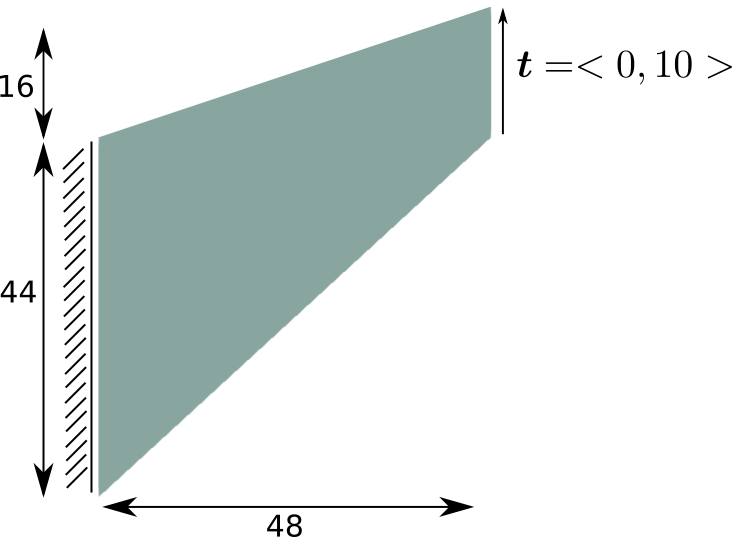
\includegraphics[width=0.4\textwidth]{img/mech_cooks_geom.png}
\caption{Cook's membrane problem definition.}
\label{fig:cooks_geom}
\end{figure}

For each QoI, an initial mesh with a uniform size of $H=8$
was generated. Figures \ref{fig:mech_cooks_pw_meshes} and
\ref{fig:mech_cooks_avg_u_meshes} show the initial mesh utilized for both
the point-wise and average displacement QoIs. From these initial meshes,
the steps
%
\begin{gather*}
\text{Solve primal PDE} \rightarrow
\text{Solve adjoint PDE} \rightarrow
\text{Localize error} \rightarrow
\text{Adapt mesh}
\end{gather*}
%
were iteratively performed until a final mesh with about $10,000$ degrees
of freedom was produced. During each mesh adaptation, the size field was
specified according to the equation \eqref{eq:mech_size_field} such that
the desired number of elements $N$ in the output mesh is twice the number
of elements in the previous mesh.

\begin{figure}[ht!]
\centering
\begin{subfigure}{.33\textwidth}
\centering
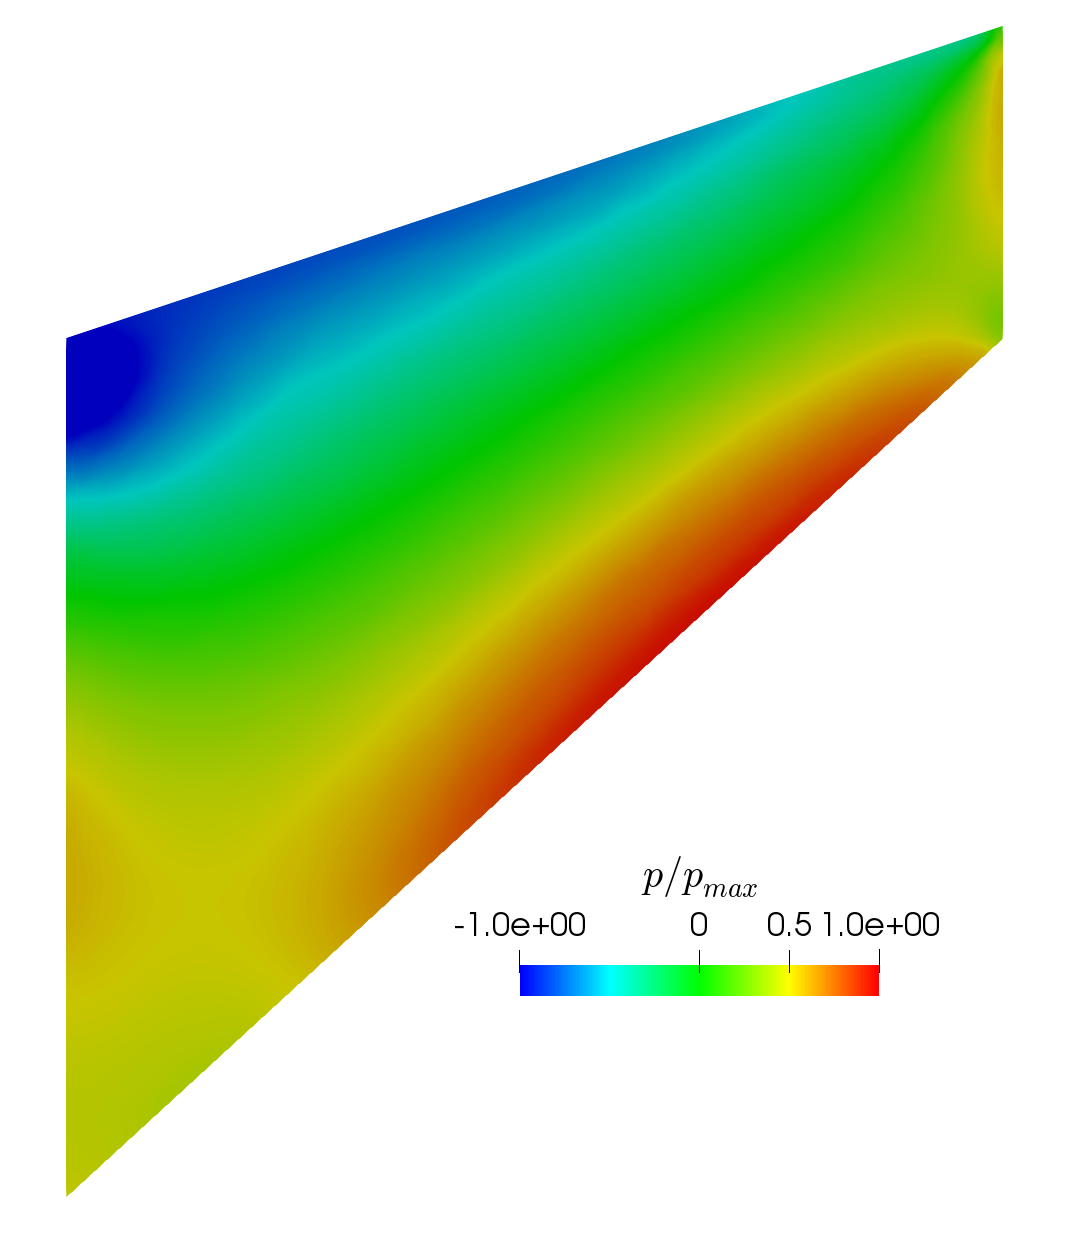
\includegraphics[width=.9\linewidth]{img/mech_cooks_pw_p.png}
\end{subfigure}%
\begin{subfigure}{.33\textwidth}
\centering
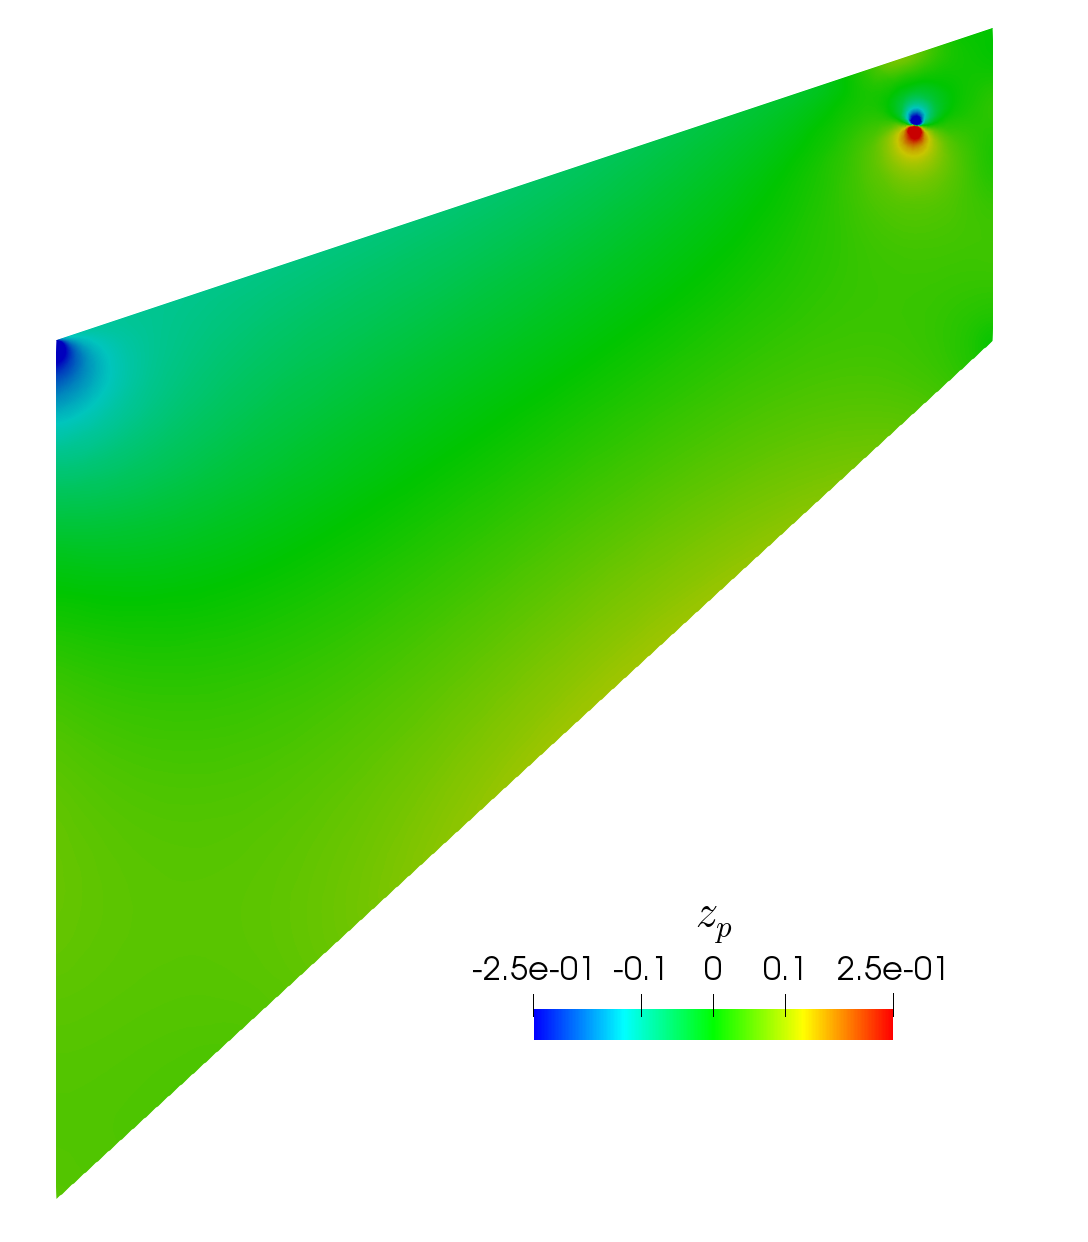
\includegraphics[width=.9\linewidth]{img/mech_cooks_pw_zp.png}
\end{subfigure}
\begin{subfigure}{.33\textwidth}
\centering
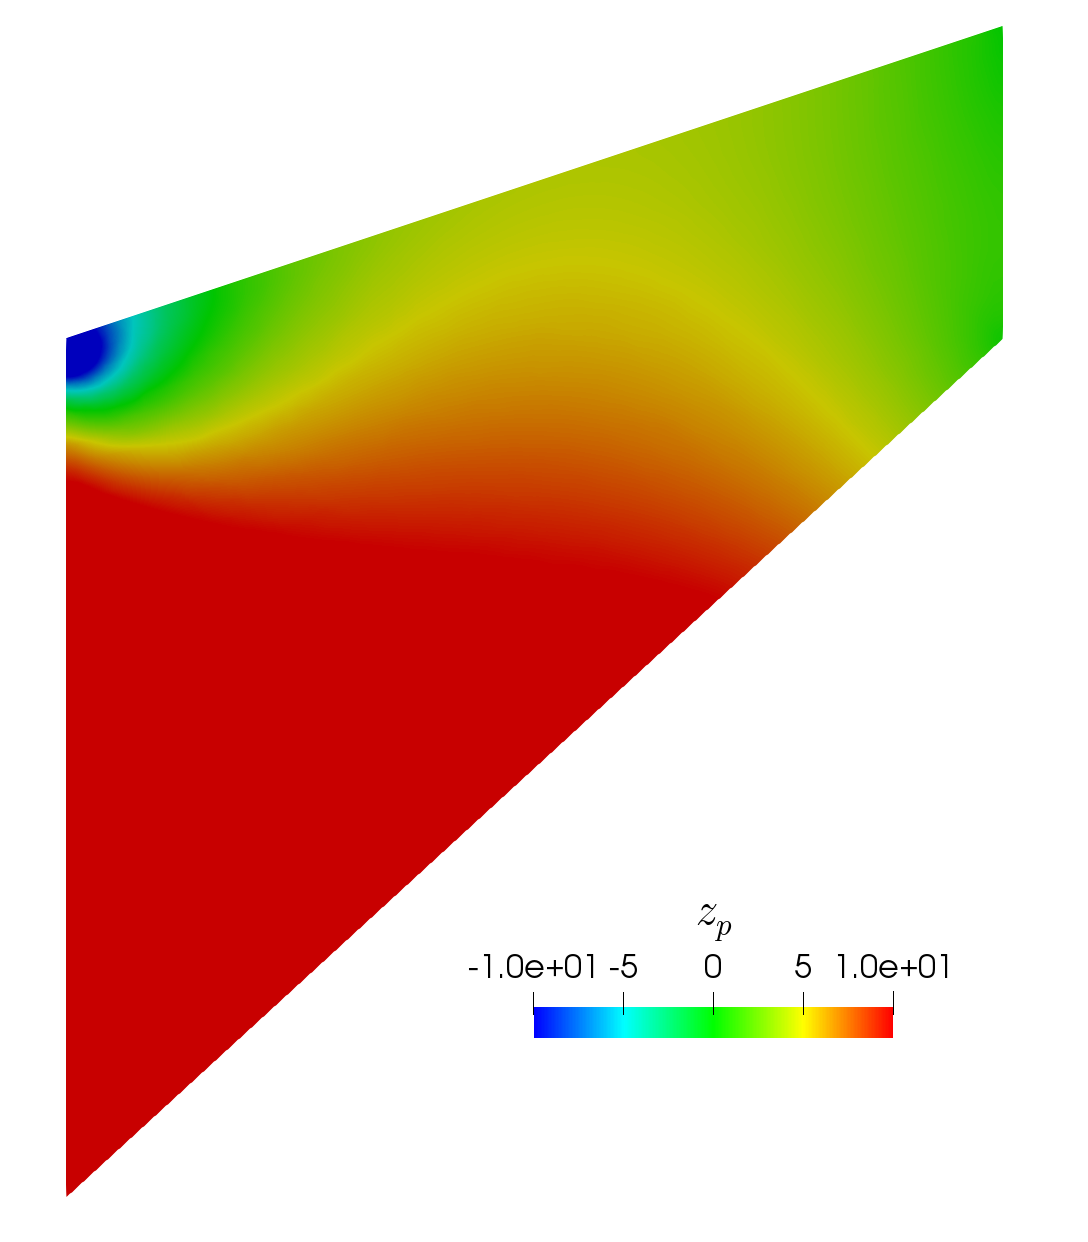
\includegraphics[width=.9\linewidth]{img/mech_cooks_avg_u_zp.png}
\end{subfigure}
\caption{The pressure component $p$ of the primal solution scaled by its
maximal value (left), the pressure component $z_p$ of the adjoint solution for
the point-wise QoI $J_1(\bs{U})$, and the pressure component $z_p$ of the
adjoint solution for the average displacement QoI $J_2(\bs{U})$.}
\label{fig:mech_cooks_pressures}
\end{figure}

The left-most figure of Figure \ref{fig:mech_cooks_pressures} illustrates
the pressure component $p$ of the primal solution scaled by its maximal
value. We remark that this result is consistent with previous literature
\cite{ostien2016tet}. The center and right-most figures of Figure
\ref{fig:mech_cooks_pressures} shows the pressure component $z_p$ of the
adjoint solution for the point-wise QoI $J_1(\bs{U})$ and the average
displacement QoI $J_2(\bs{U})$, respectively. For the point-wise QoI, the
adjoint solution $z_p$ is highly localized to the point that defines the
QoI and the corner of stress singularity.

\begin{figure}[ht!]
\centering
\begin{subfigure}{.5\textwidth}
\centering
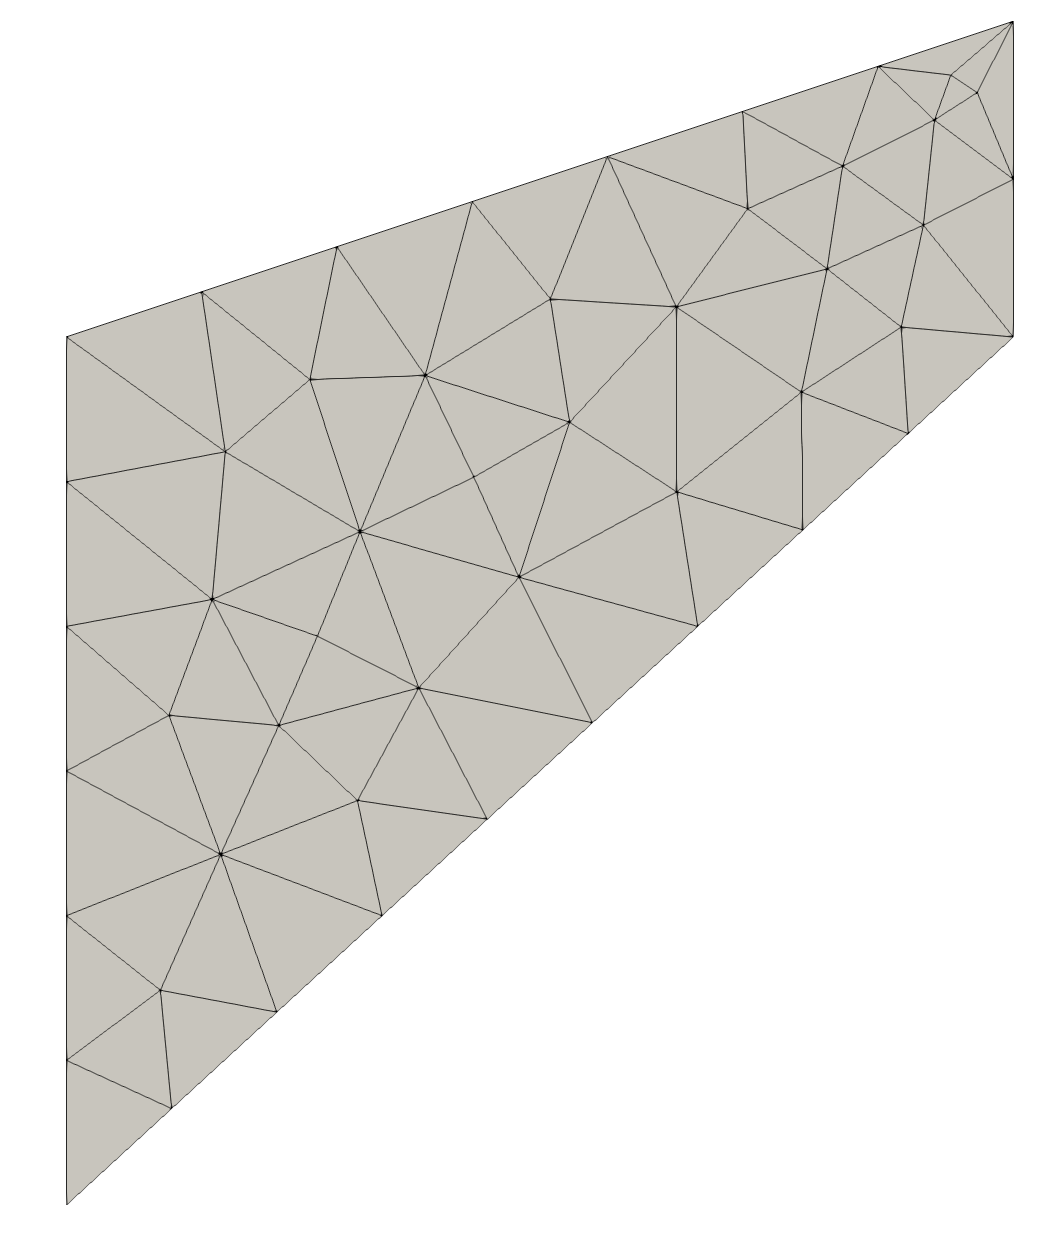
\includegraphics[width=.6\linewidth]{img/mech_cooks_pw_initial_mesh.png}
\end{subfigure}%
\begin{subfigure}{.5\textwidth}
\centering
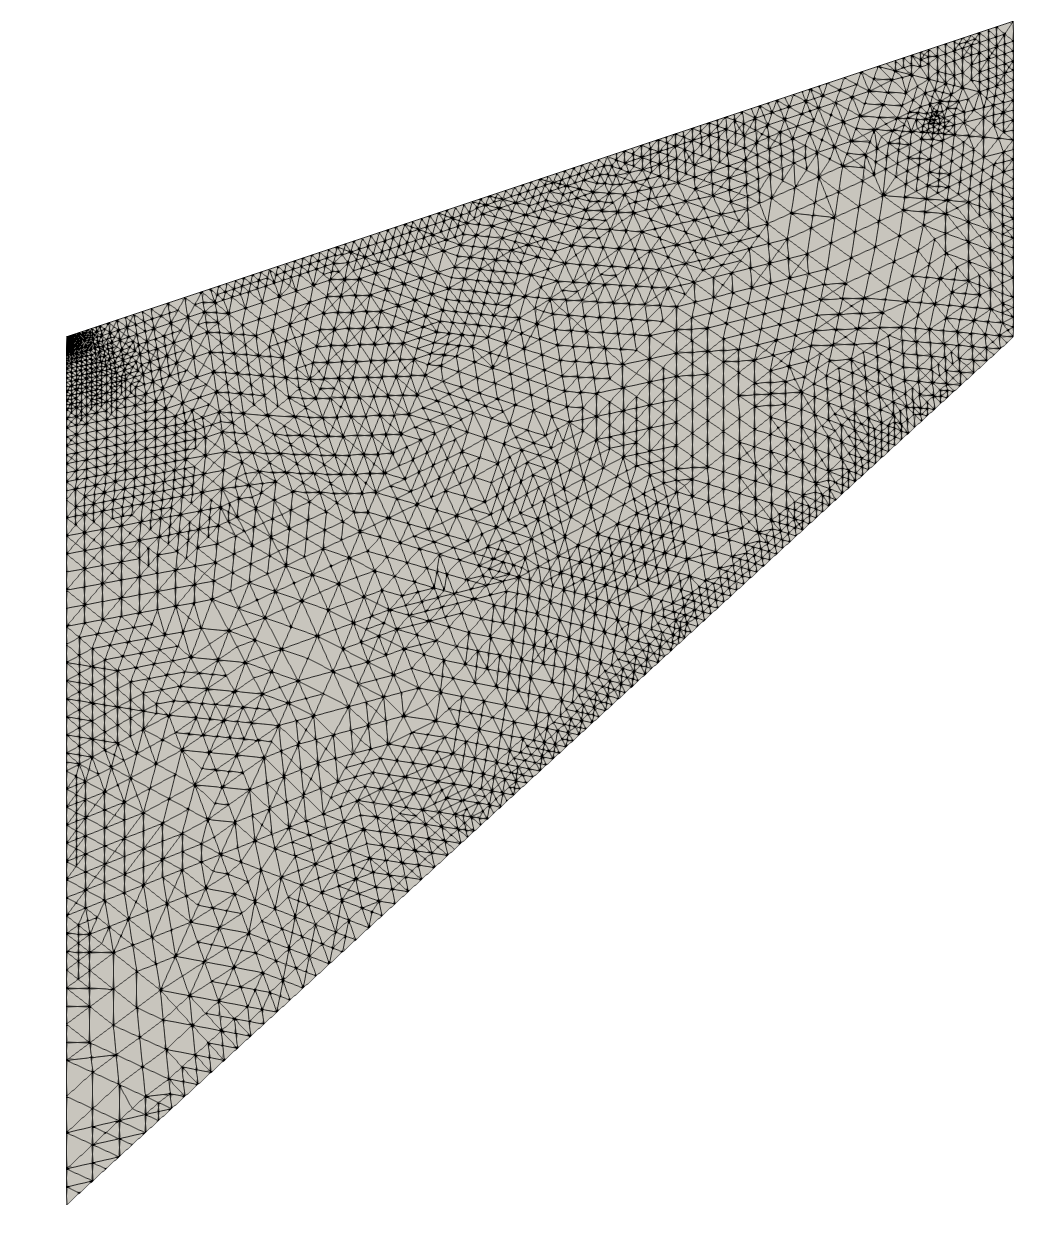
\includegraphics[width=.6\linewidth]{img/mech_cooks_pw_final_mesh.png}
\end{subfigure}
\caption{Initial mesh (left) and adapted mesh (right) at the fifth
adaptive iteration for the Cook's membrane problem with the point-wise
QoI $J_1(\bs{U})$.}
\label{fig:mech_cooks_pw_meshes}
\end{figure}

To approximate the exact values of the quantities of interest, the primal
problem was solved on a ``truth'' mesh with about $1.5$ million degrees of
freedom. This mesh is finer at every spatial location than the final meshes
produced by the two adaptive simulations. The reference value for the
point-wise QoI on the truth mesh was computed to be
$J_1(\bs{U}) = 2.395627$ and the reference value for the average displacement
QoI was computed to be $J_2(\bs{U}) = 324.0948$.

\begin{figure}[ht!]
\centering
\begin{subfigure}{.5\textwidth}
\centering
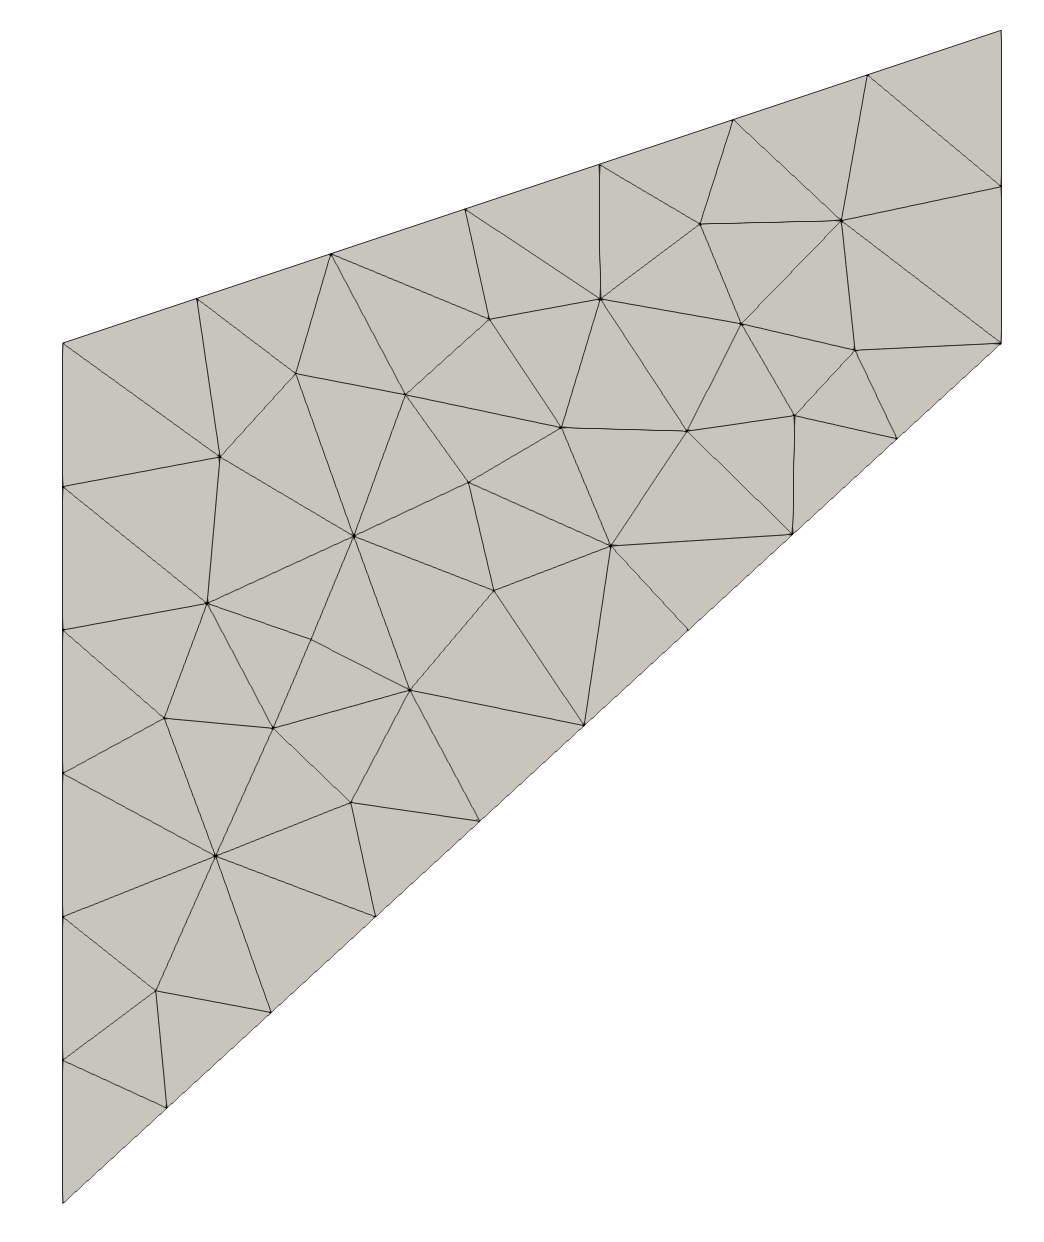
\includegraphics[width=.6\linewidth]{img/mech_cooks_avg_u_initial_mesh.png}
\end{subfigure}%
\begin{subfigure}{.5\textwidth}
\centering
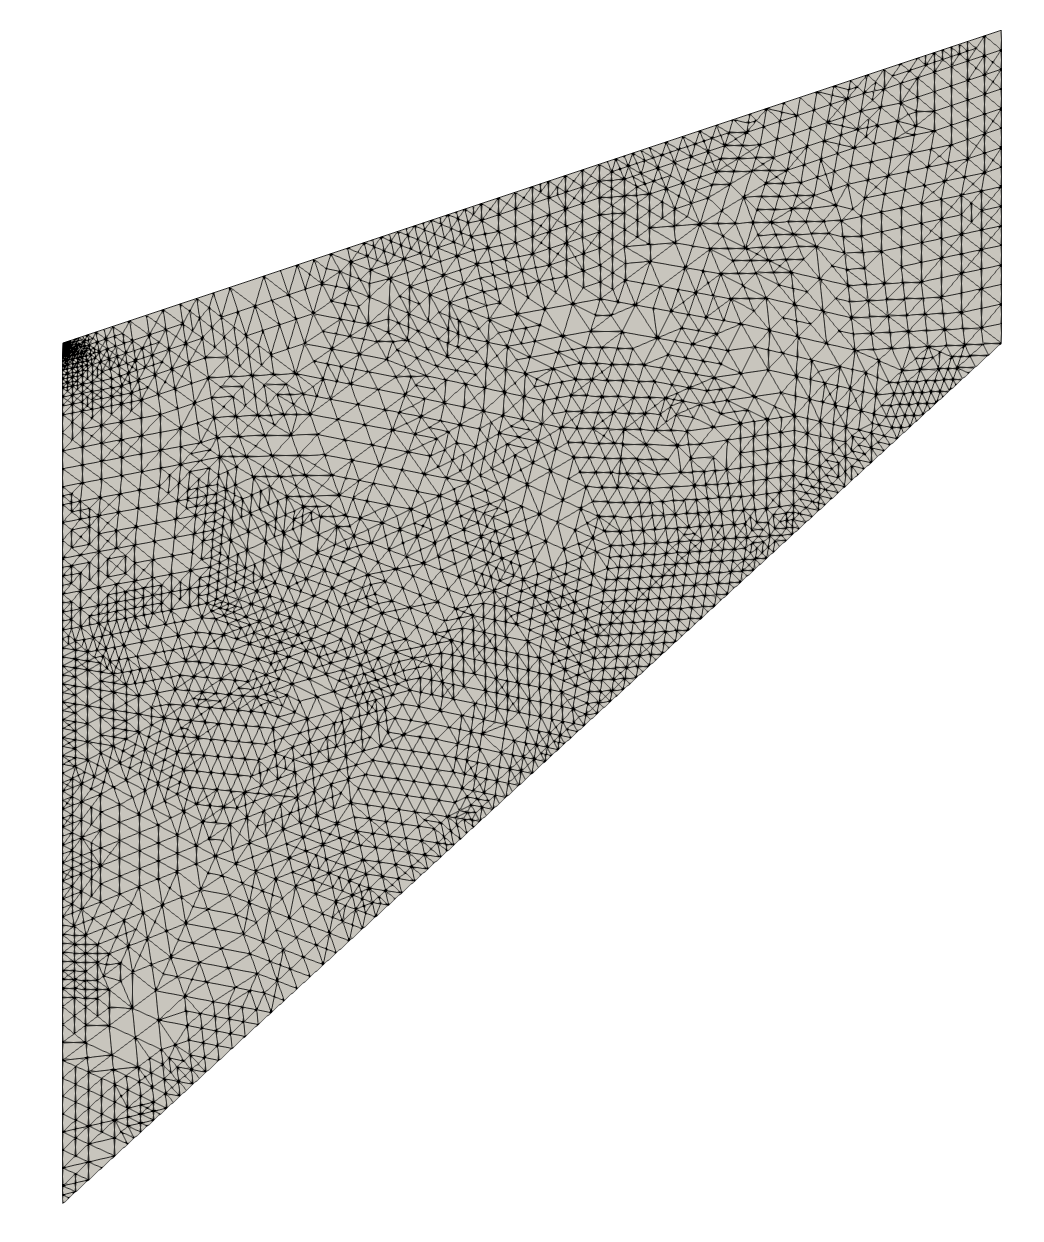
\includegraphics[width=.6\linewidth]{img/mech_cooks_avg_u_final_mesh.png}
\end{subfigure}
\caption{Initial mesh (left) and adapted mesh (right) at the fifth adaptive
iteration for the Cook's membrane problem with the average displacement
QoI $J_2(\bs{U})$.}
\label{fig:mech_cooks_avg_u_meshes}
\end{figure}

We consider two different errors, the ``exact error'' $\E = J(\bs{U}) -
J^h(\bs{U}^h_H)$ and the error $\E_h = J^h(\bs{U}^h) - J^h(\bs{U}^h_H)$
with respect to the functional evaluated on the fine mesh with mesh size
$\frac{H}{2}$. Here we place quotations around the term ``exact error''
because we have only approximated $J(\bs{U})$ with high fidelity and have
not obtained its actual exact value. We recall the effectivity index
\eqref{eq:mech_effectivity} defined as $\I = \frac{\eta}{\E}$ and additionally
define a discrete effectivity index as $I_h = \frac{\eta}{\E_h}$. An
effecitivty index of $\I = 1$ indicates that the error estimate $\eta$ has
exactly recovered the ``true error''. Similarly, a discrete effectivity index
of $\I_h = 1$ indicates that the error estimate $\eta$ has exactly recovered
the error between the functional evaluated on the fine space and the
functional evaluated on the coarse space. Figure
\ref{fig:mech_cooks_effectivity} plots the effectivity $\I$ relative to the
``exact error'' and the effectivity $\I_h$ relative to the fine-space error,
and demonstrates the ability of $\eta$ to effectively estimate the error as
$H \to 0$ during the adaptive process for the chosen functional quantities.
The small distance away from $1$ in the discrete effectivity index $\I_h$
represents the linearization error associated with the estimate $\eta$,
introduced by the linearized adjoint problem \eqref{eq:mech_adjoint_problem}.


\begin{figure}[ht!]
\centering
\begin{subfigure}{.5\textwidth}
\centering
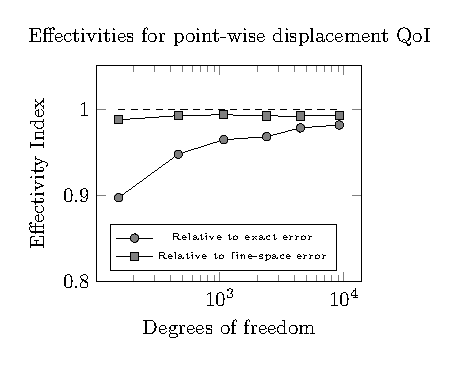
\includegraphics[width=.99\linewidth]{img/mech_cooks_pw_effectivity_plot.pdf}
\end{subfigure}%
\begin{subfigure}{.5\textwidth}
\centering
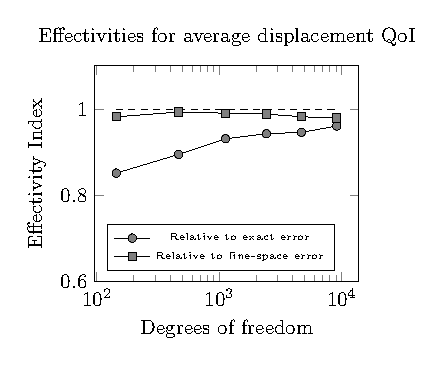
\includegraphics[width=.95\linewidth]{img/mech_cooks_avg_disp_effectivity_plot.pdf}
\end{subfigure}
\caption{Effectivities for the point-wise QoI $J_1(\bs{U})$ (left) and for the
average displacement QoI $J_2(\bs{U})$ (right) for the Cook's membrane
problem.}
\label{fig:mech_cooks_effectivity}
\end{figure}

Figure \ref{fig:mech_cooks_error} demonstrates the evolution of various errors
throughout the adaptive process. First, we note that the ``exact error'' $\E$
and the estimated error $\eta$ are very close, as previously discussed. Next,
we note that the estimated bound $\hat{\eta}$ on the functional error,
computed as the sum of localized error contributions, overestimates the error,
but only by a small factor. This provides some justification to expect that
the derived correction indicators are well-suited to drive mesh adaptation.
Finally, we remark that an improved corrected functional value
$J^*(\bs{U}^h_H)$ can be computed as the approximated functional value plus
the estimated error, $J^*(\bs{U}^h_H) = J^h(\bs{U}^h_H) + \eta$. This
corrected value tends to converge at a faster rate than the computed value
$J^h(\bs{U}^h_H)$. In particular, this corrected value can prove valuable
for coarser discretizations, where the error in the corrected value is
around two orders of magnitude smaller than the error in the computed
value of the functional.

\begin{figure}[ht!]
\centering
\begin{subfigure}{.5\textwidth}
\centering
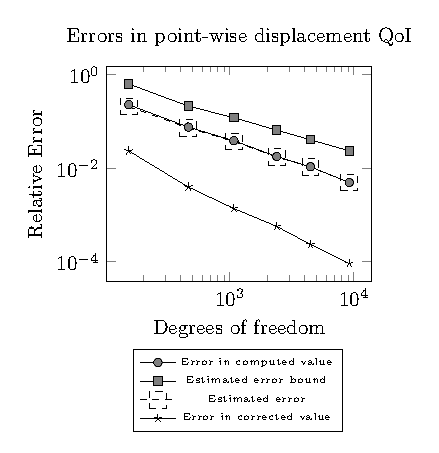
\includegraphics[width=.99\linewidth]{img/mech_cooks_pw_error_plot.pdf}
\end{subfigure}%
\begin{subfigure}{.5\textwidth}
\centering
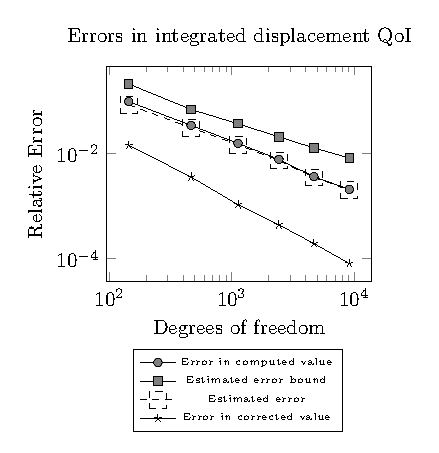
\includegraphics[width=.95\linewidth]{img/mech_cooks_avg_disp_error_plot.pdf}
\end{subfigure}
\caption{Errors for the point-wise QoI $J_1(\bs{U})$ (left) and for the
average displacement QoI $J_2(\bs{U})$ (right) for the Cook' membrane problem.}
\label{fig:mech_cooks_error}
\end{figure}

Figure \ref{fig:mech_cooks_pw_meshes} shows the adapted mesh after $5$
adaptive cycles for the point-wise QoI. We first note that the mesh is
heavily refined in the upper left corner of the mesh, where there is a stress
singularity. Without accurately resolving this singularity, so-called
``pollution error'' \cite{babuvska1994pollution}
will affect the accuracy of the finite element solution
throughout the domain. This demonstrates that the adaptive adjoint-based
procedure accurately identifies other sources of error that must be resolved
even when a fully localized QoI is chosen. Similarly, Figure
\ref{fig:mech_cooks_avg_u_meshes} shows the adapted mesh after $5$
adaptive cycles for the average displacement QoI. Again there is heavy
refinement in the corner with the stress singularity.

Interestingly, Figure \ref{fig:mech_cooks_pw_meshes} also illustrates that
the adjoint-based adaptive procedure refines around the spatial location
that defines the point-wise QoI. This may, in part, be explained by the fact
that the data driving the adjoint problem is a discrete delta function.
However, such refinement is unlikely to lead to an optimal distribution of
degrees of freedom in the mesh. In essence, the Cook's membrane problem
is a cantilever beam and this result indicates that we must refine
heavily at the end of the beam in order to accurately evaluate displacements
at the beam tip. This is antithetical to engineering intuition and
experience. Another factor leading to this result may be our choice of
error localization. We have localized the error based on a PU-based weak
form statement \eqref{eq:mech_error_localization}, where derivatives are left
on the weighting function term $\bs{Z}$. This, in turn, may lead to a
heavier emphasis on the local point-wise location during the adaptive
process. We leave investigation into this area as an avenue for future
study.

%%% A CELL EMBEDDED IN A MATRIX
\subsection{A Cell Embedded in a Matrix}

In this section, we apply adjoint-based error estimation and mesh adaptation
to a three-dimensional problem that arises in the study of cellular
biomechanics and mechanobiology. The problem of interest involves
investigating a cell embedded in an extracellular matrix. The traction that
this cell exerts on its surroundings directly influences cellular processes
like migration and differentiation. Recently, Dong and Oberai
\cite{dong2017recovery} introduced a process to recover cellular tractions
based on the solution of an \emph{inverse} problem. For this inverse problem,
it is assumed that displacements throughout the extracellular matrix are given
with some uncertainty, and successive solutions of a \emph{forward} problem are
solved to recover the tractions driving the problem. Presently, we focus on
accurately solving the forward problem in this process using adjoint-based
error estimation. That is, given tractions imposed on the cellular membrane,
we would like to solve for displacements in some region of the domain as
accurately as possible. 

\begin{figure}[ht!]
\centering
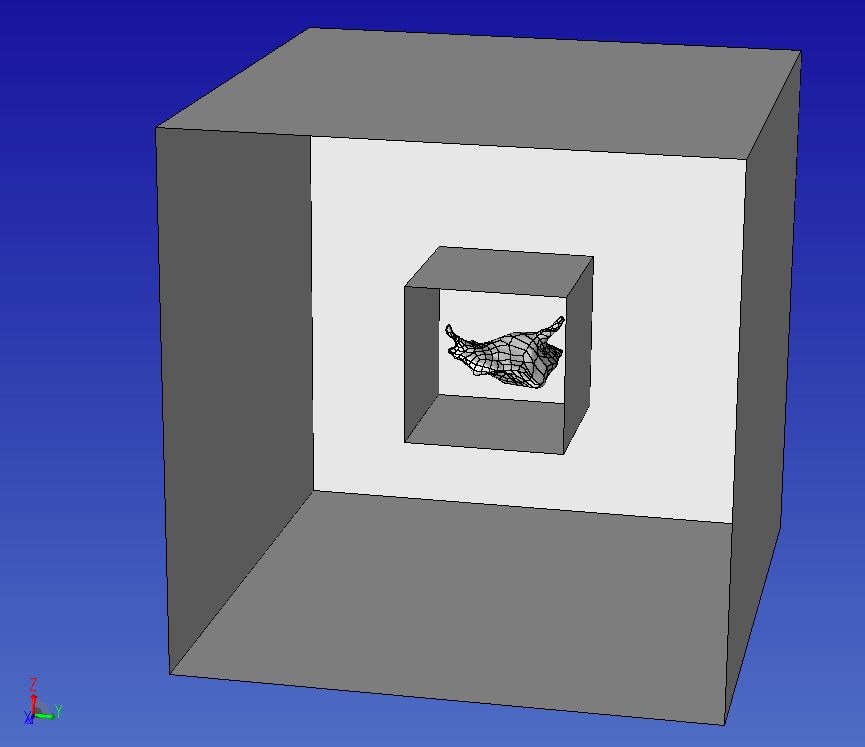
\includegraphics[width=.6\linewidth]{img/mech_glial_geom.png}
\centering
\caption{The computational geometry for the microglial cell problem. The
inner-most surface represents the geometry of the microgial cell, the
outer-most bounding box represents the extracellular matrix in which the
cell is embedded, and the inner bounding box represents the domain over
which the local average displacement QoI $J(\bs{U})$ is defined.}
\label{fig:mech_glial_geom}
\end{figure}

Specifically, we focus on a microglial cell with dimensions of about
$20 \mu m \times 20 \mu m \times 20 \mu m$ embedded in an extracellular matrix
of dimension $100 \mu m \times 100 \mu m \times 100 \mu m$. We choose the
QoI to be a local average displacement,
$J(\bs{U}) = \int_{\B_0} \frac13 (u_x + u_y + u_z) \, \text{d} V$, defined
over a $30 \mu m \times 30 \mu m \times 30 \mu m$ bounding box $\B_0$
surrounding the microglial cell. Figure \ref{fig:mech_glial_geom} shows the
geometry defining the microglial cell, the extracellular matrix, and the
local QoI domain $\B_0$. For the extracellular matrix,
the shear modulus $\mu = \frac{E}{2(1 + \nu)}$ is set to be 600 Pa and
Poisson's ratio is set to be $\nu = 0.4999$, which is consistent with
material properties for hydrogels
\cite{legant2010measurement, paszek2005tensional, discher2005tissue}.

\begin{figure}[ht!]
\centering
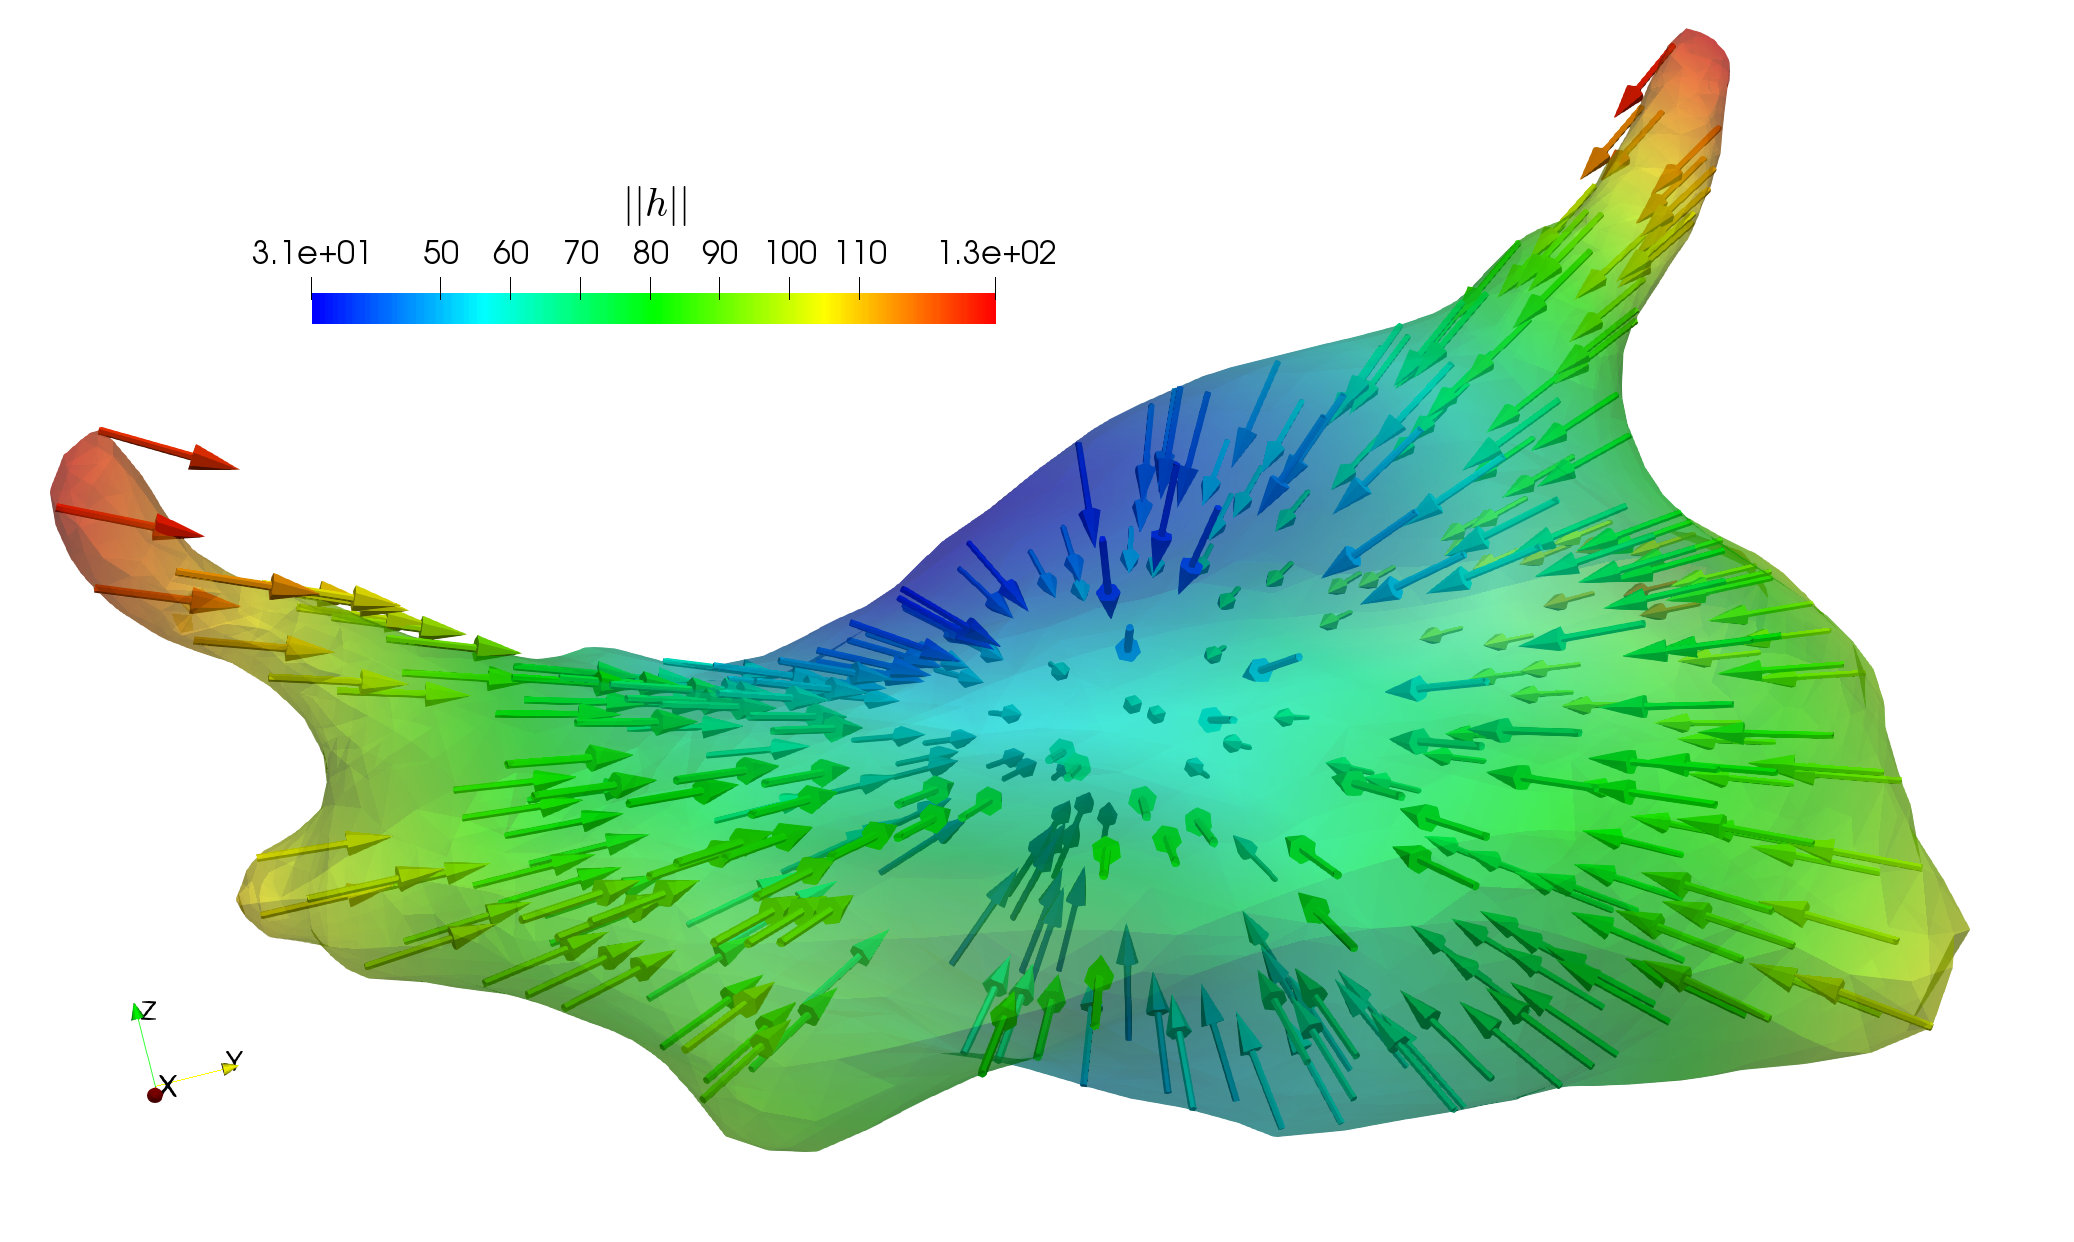
\includegraphics[width=.6\linewidth]{img/mech_glial_applied_traction.png}
\centering
\caption{The applied tractions for the microglial cell problem.}
\label{fig:mech_glial_traction}
\end{figure}

To drive the problem, we impose traction boundary conditions along the
surface of the microglial cell. The magnitude of the traction $\bs{h}$ is
defined to be 10 times the distance to the center of the microglial cell and
its direction points inward toward the center of the microglial cell. The
applied traction is shown in Figure \ref{fig:mech_glial_traction}. This
traction serves to pull the extracellular matrix inwards towards the center
of the microglial cell, which is consistent with observed physical behavior
\cite{dong2017recovery}. The deformation of the cell surface due to this
applied traction is shown in Figure \ref{fig:mech_glial_deformed}. To
constrain rigid body translations and rotations, we prescribe displacements
$u_x = 0$ on the face with constant minimum $x$-coordinate value, $u_y = 0$
on the face with constant minimum $y$-coordinate value, and $u_z = 0$ on the
face with constant minimum $z$-coordinate value. As a reference value for
the average displacement QoI, the primal problem was solved on a ``truth''
mesh with about $60$ million degrees of freedom. The reference value for the
QoI was computed to be $J(\bs{U}) = -527.1453$.

\begin{figure}[ht!]
\centering
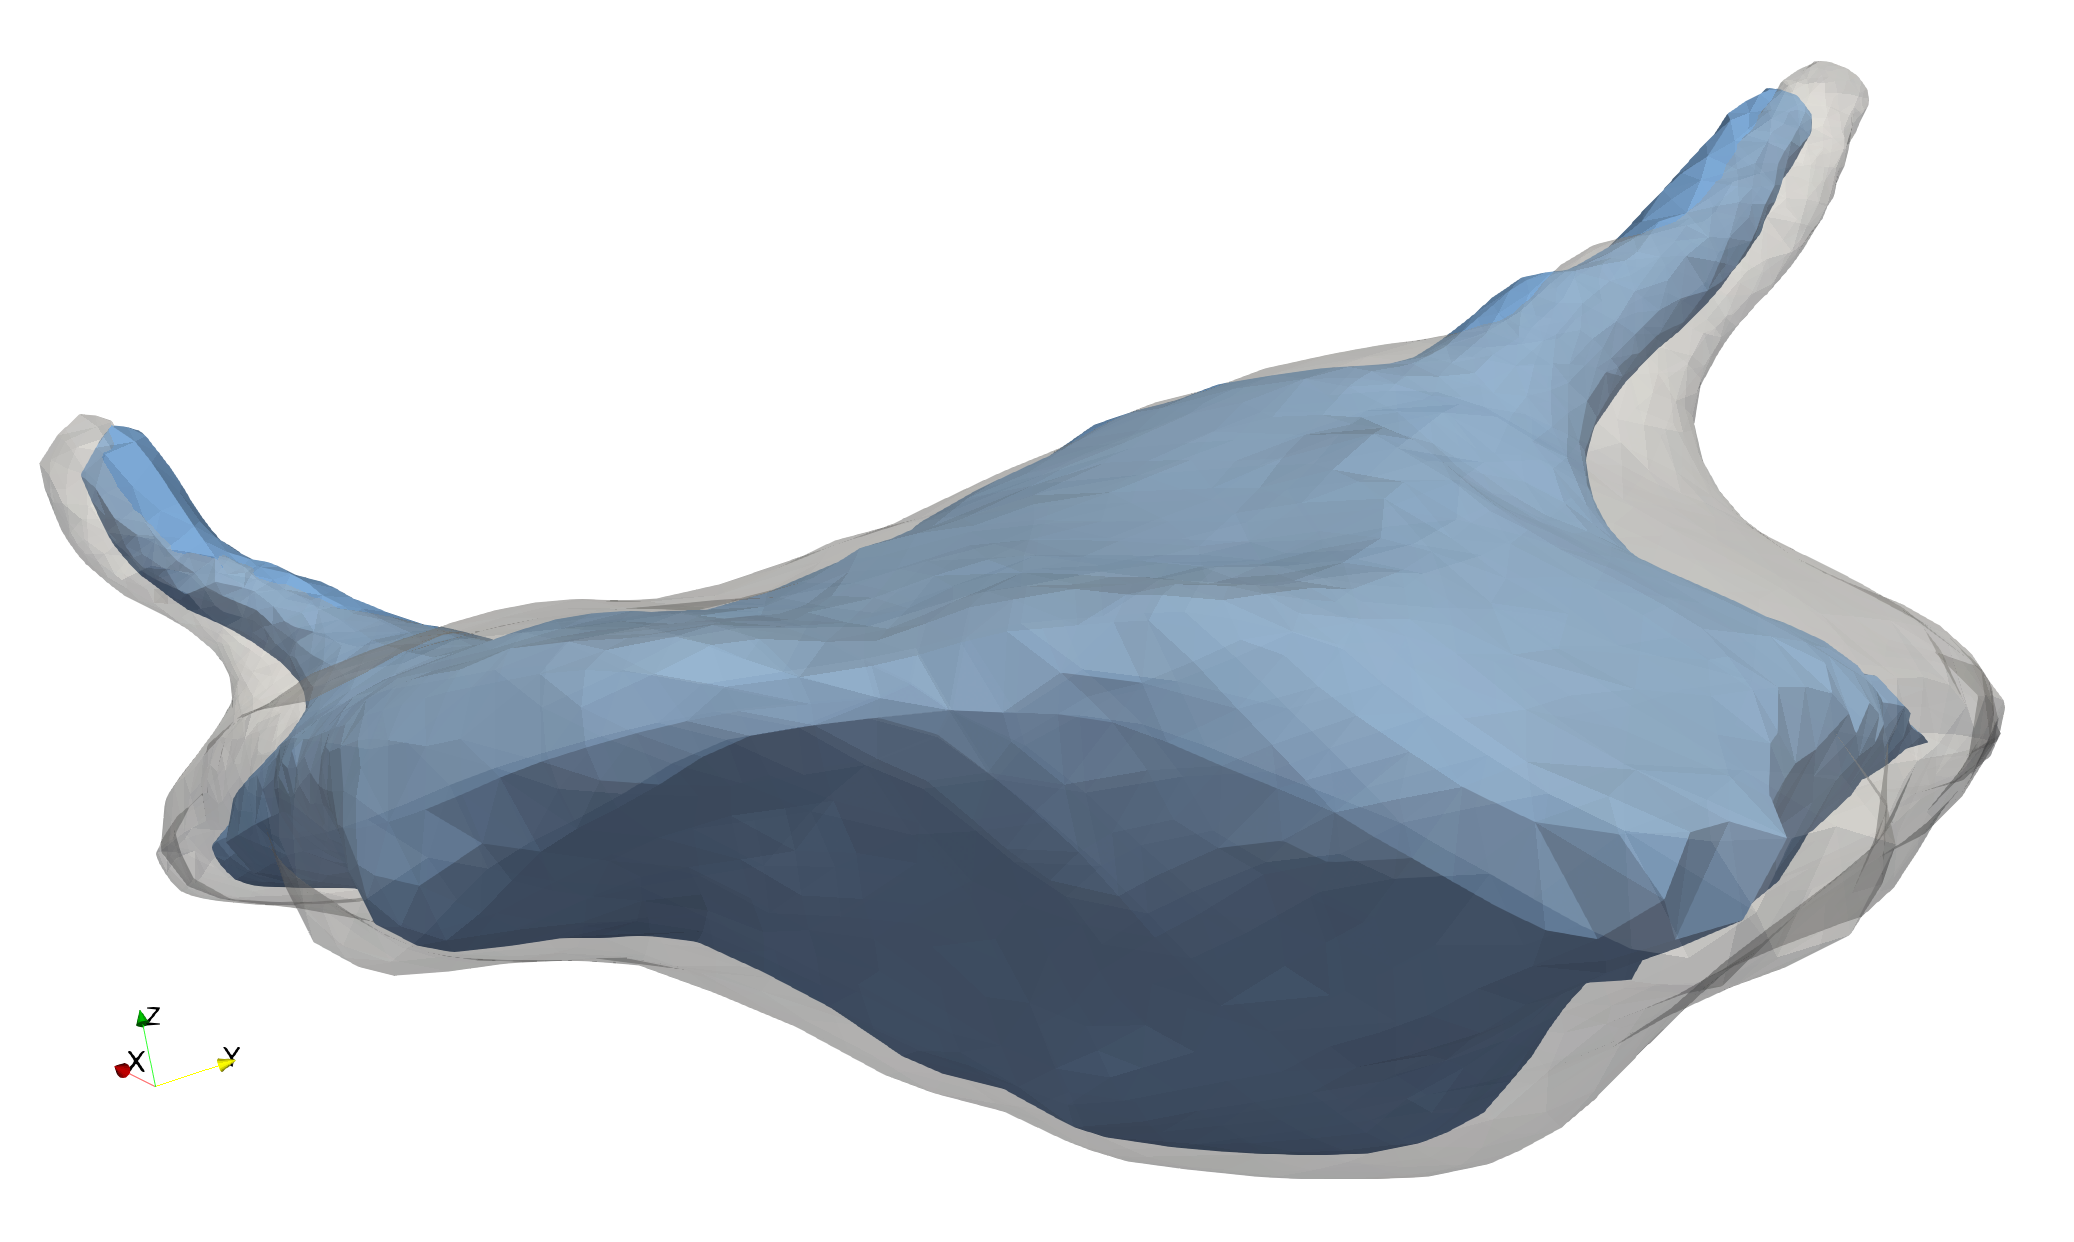
\includegraphics[width=.6\linewidth]{img/mech_glial_deformed.png}
\caption{The initial (light grey) and deformed (blue) geometry of the
microglial cell before and after tractions are applied.}
\label{fig:mech_glial_deformed}
\end{figure}

\begin{figure}[ht!]
\centering
\begin{subfigure}{.5\textwidth}
\centering
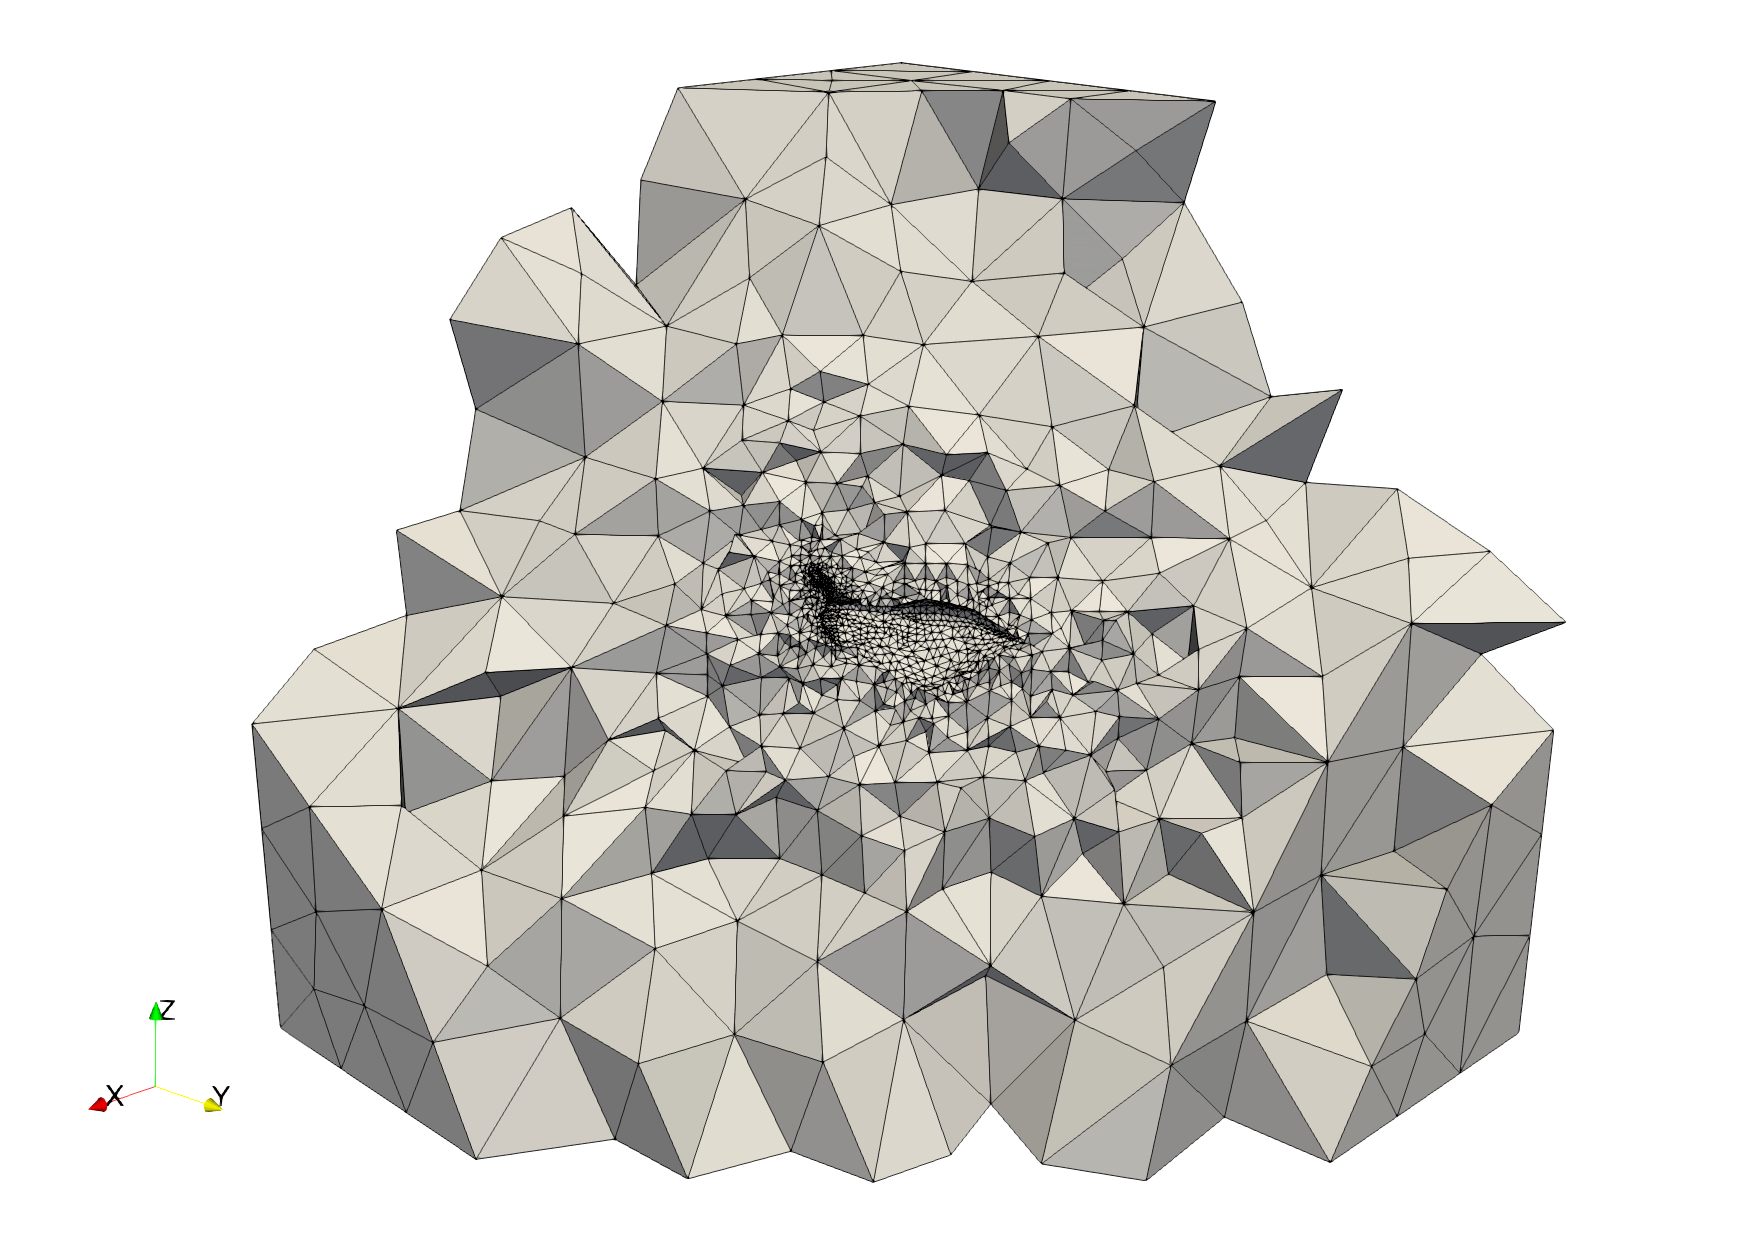
\includegraphics[width=.99\linewidth]{img/mech_glial_initial_mesh.png}
\end{subfigure}%
\begin{subfigure}{.5\textwidth}
\centering
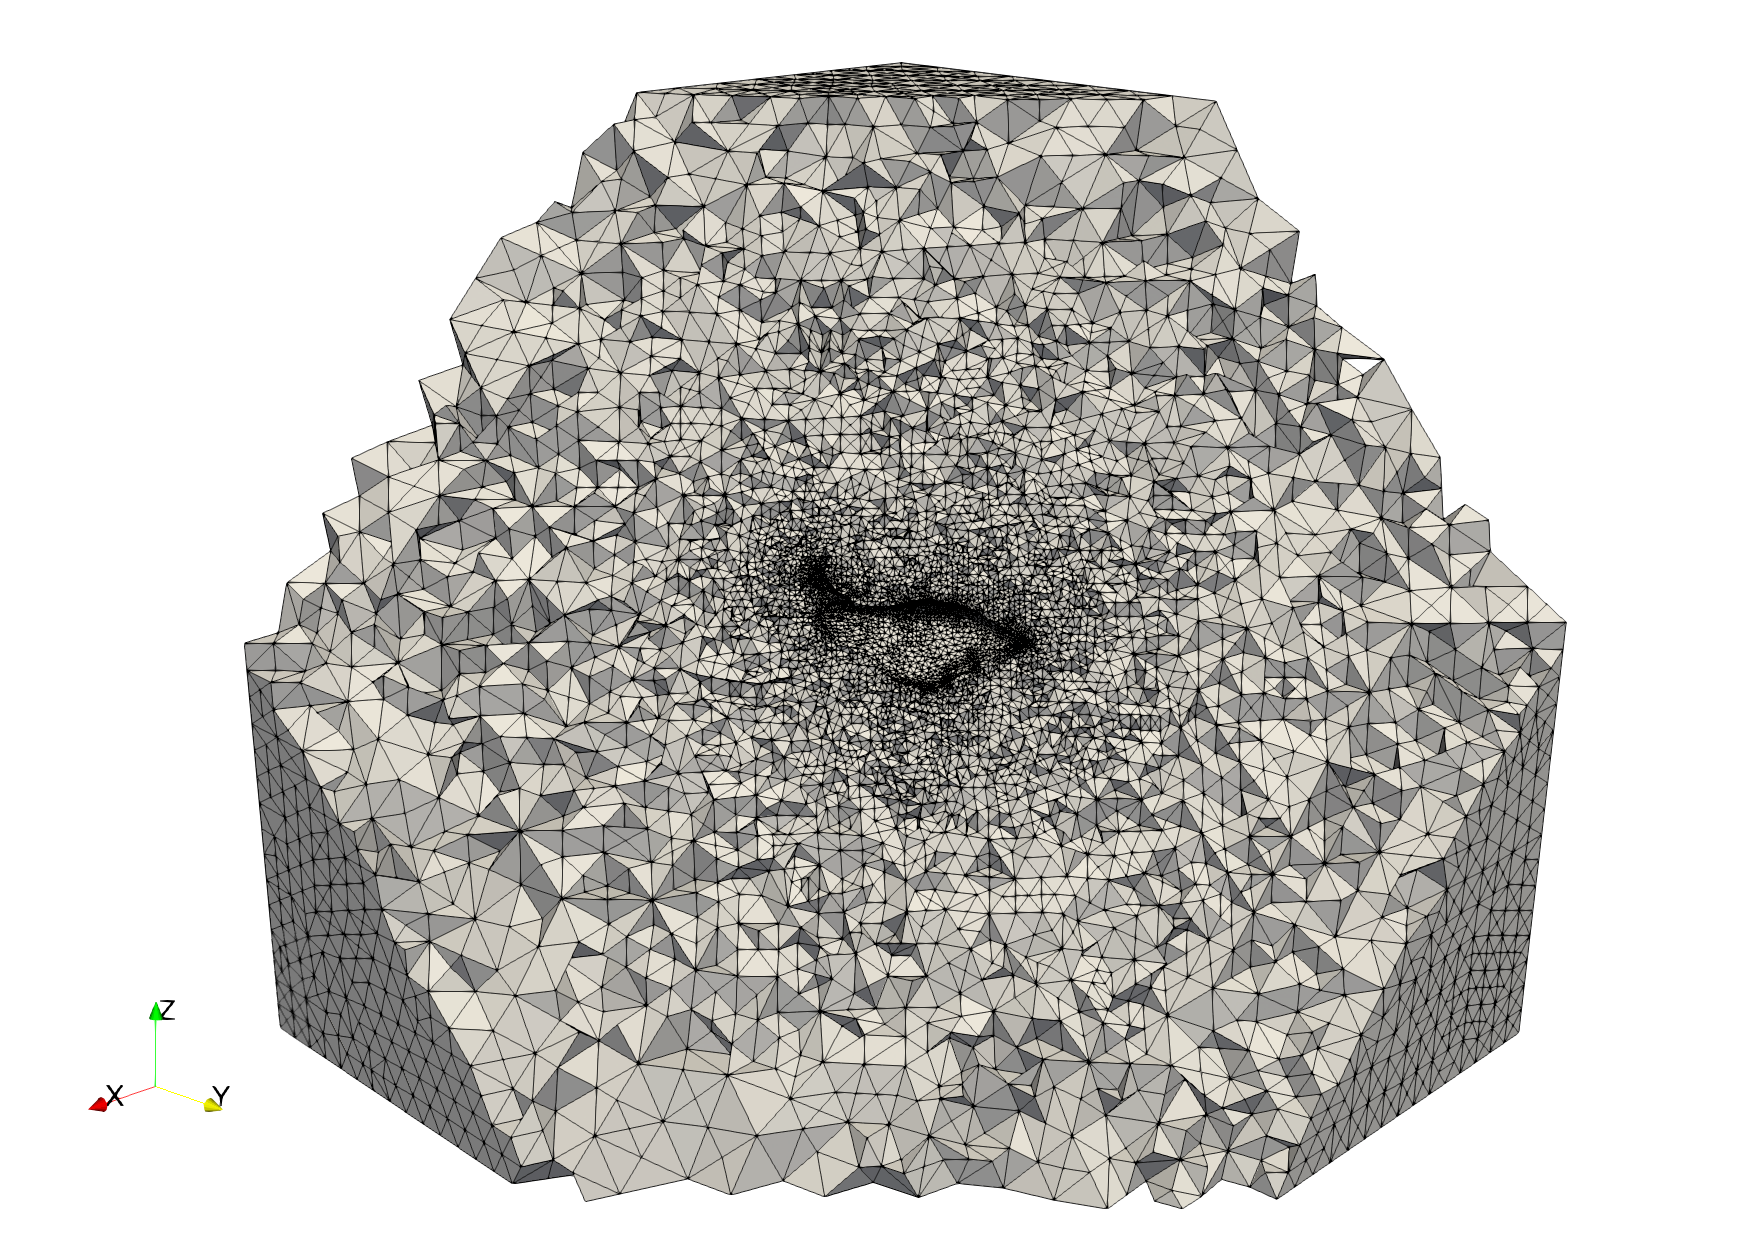
\includegraphics[width=.99\linewidth]{img/mech_glial_final_mesh.png}
\end{subfigure}
\caption{Initial mesh for the microglial cell problem (left) and final adapted
mesh after $10$ adaptive iterations (right).}
\label{fig:mech_glial_meshes}
\end{figure}

An initial mesh with about $30,000$ degrees of freedom was generated, as
shown in Figure \ref{fig:mech_glial_meshes}. From this initial mesh, the
steps
%
\begin{gather*}
\text{Solve primal PDE} \rightarrow
\text{Solve adjoint PDE} \rightarrow
\text{Localize error} \rightarrow
\text{Adapt mesh}
\end{gather*}
%
were iteratively performed $10$ times.  The mesh size field was specified
according to equation \eqref{eq:mech_size_field} such that the desired number
of elements $N$ in the output mesh is $1.5$ times the number of elements in
the previous mesh.

\begin{figure}[ht!]
\centering
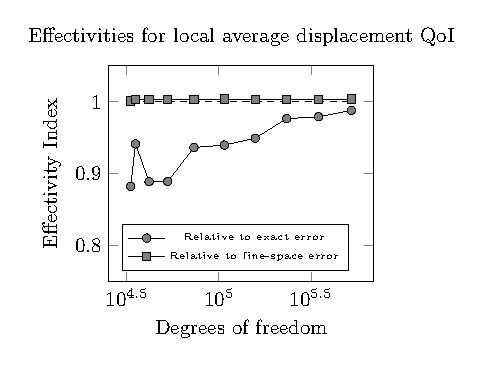
\includegraphics[width=.5\linewidth]{img/mech_glial_effectivity_plot.pdf}
\caption{Effectivity indices for the local average displacement QoI
$J(\bs{U})$ for the microglial cell problem.}
\label{fig:mech_glial_effectivity}
\end{figure}

We again consider the ``exact error'' $\E = J(\bs{U}) - J^h(\bs{U}^h_H)$ and
the error $\E_h = J^h(\bs{U}^h) - J^h(\bs{U}^h_H)$ with respect to the
functional evaluated on the fine mesh, and their effectivity indices
$\I = \frac{\eta}{\E}$ and $I_h = \frac{\eta}{\E_h}$, respectively. Here
$\eta$ denotes the error estimate computed by \eqref{eq:mech_error_estimate}.
We again expect that the functional will converge at the rate $k = 2$ and use
the correction value $\alpha = \frac34$.

Figure \ref{fig:mech_glial_effectivity} plots the effectivity index $\I$
relative to the ``exact error'' and the effectivity index $I_h$ relative to the
fine space error. The small distance away from $1$ in the discrete effectivity
index $\I_h$ is associated with the linearization error introduced by the
adjoint problem. Additionally, the ability of the error estimate to recover
the ``exact error'' as $H \to 0$ compared to the reference value is
demonstrated by the effectivity $\I$.

\begin{figure}[ht!]
\centering
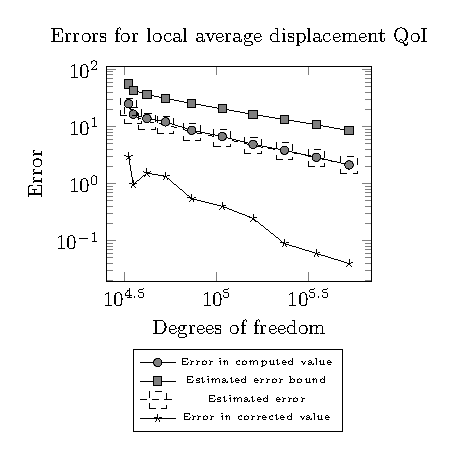
\includegraphics[width=.5\linewidth]{img/mech_glial_error_plot.pdf}
\caption{Errors for the local average displacement QoI $J(\bs{U})$ for the
microglial cell problem.}
\label{fig:mech_glial_error}
\end{figure}

\begin{figure}[ht!]
\centering
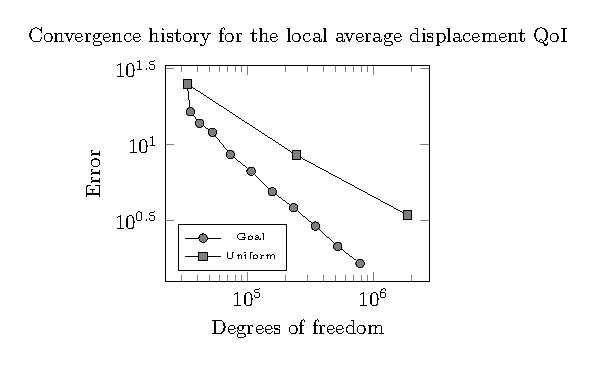
\includegraphics[width=.6\linewidth]{img/mech_glial_convergence_plot}
\caption{Error convergence using uniform mesh refinement (Uniform) and
adjoint-based adaptivity (Goal) for the local average displacement QoI
$J(\bs{U})$ for the microglial cell problem.}
\label{fig:mech_glial_convergence}
\end{figure}

Figure \ref{fig:mech_glial_error} displays the evolution of various errors
throughout the adaptive process. In particular, the ``exact error'' $\E$ and
the estimated error $\eta$ are very close, as previously noted by the
effectivity index $\I$. As for the Cook's membrane problem the estimated error
bound $\hat{\eta}$ overestimates the error, but not to a drastic degree.
Finally, we remark that the corrected functional value, computed as
$J^*(\bs{U}^h_H) = J^h(\bs{U}^h_H) + \eta$, is nearly two orders of magnitude
more accurate at the final adaptive step, demonstrating the usefulness
of adjoint-based error estimation.

Finally, we plot the evolution of the ``exact error'' for two adaptive
strategies in Figure \ref{fig:mech_glial_convergence}. We compare the
convergence of errors for uniform mesh refinement and the developed
adjoint-based adaptive scheme. The error is converging at a faster rate for
the adjoint-based adaptive scheme. Further, the adjoint-based adaptive scheme
achieves the same accuracy as the uniform refinement scheme with nearly an
order of magnitude fewer degrees of freedom at around $110,000$ degrees
freedom. This demonstrates the utility of adjoint-based adaptivity for solid
mechanics problems.

%%% CONCLUSIONS
\section{Conclusions}

In this chapter, we have developed an adjoint-based error estimation
procedure for nonlinear finite deformation elasticity using a stabilized
finite element method, where we have utilized a recently developed PU-based
error localization strategy. We have demonstrated the ability of this approach
to accurately estimate functional errors for a two-dimensional model
problem. Further, we have demonstrated the utility of adaptive adjoint-based
analysis in the context of a three-dimensional example problem motivated
by the study of biological tissues. Future work includes analytically and
numerically investigating the differences in the PU-based localization
approach as compared to a more classical strong-form localization approach
for localized point-wise quantities of interest.
